\documentclass[10pt]{beamer}

\usepackage[spanish, mexico]{babel}
\usepackage[utf8]{inputenc}

\usetheme[progressbar=frametitle]{metropolis}
\usepackage{appendixnumberbeamer}

\usepackage{booktabs}
\usepackage[scale=2]{ccicons}

\usepackage{pgfplots}
\usepgfplotslibrary{dateplot}

\usepackage{xspace}
\newcommand{\themename}{\textbf{\textsc{metropolis}}\xspace}

\title{Proyecto de Grado}
\subtitle{Aprendizaje fin a fin para la conducción autónoma de vehículos domésticos usando visión artificial y redes neuronales convolucionales}
\date{\today}
% \date{}
\author{Postulante: Jose Eduardo Laruta Espejo \\ 
        Asesor: Javier Sanabria}
\institute{Universidad Mayor de San Andrés - Facultad de Ingeniería}
% \titlegraphic{\hfill\includegraphics[height=1.5cm]{logo.pdf}}

\begin{document}

\maketitle

\begin{frame}{Contenido}
  \setbeamertemplate{section in toc}[sections numbered]
  \tableofcontents[hideallsubsections]
\end{frame}

%%%
\section{Introducción}


\begin{frame}[fragile]{Planteamiento del problema}

  Un sistema de conducción autónomo cuenta con la siguiente arquitectura:
  \begin{figure}[!h] 
    \centering
    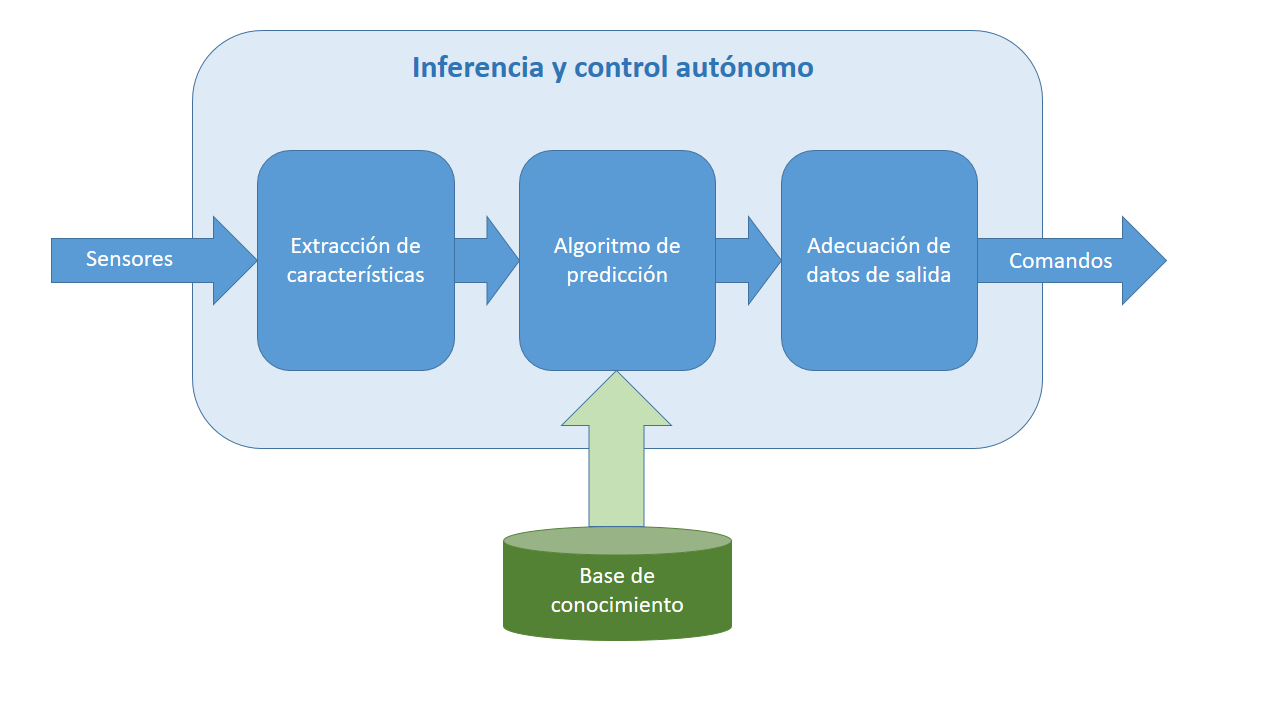
\includegraphics[width=0.75\textwidth]{../img/inferencia}
    \caption[Inferencia y control autónomo tradicional]{Componentes del subsistema de inferencia y control autónomo tradicional. Fuente: Elaboración propia.}
\end{figure}

\end{frame}

\begin{frame}[fragile]{Planteamiento del problema}

    El sistema presenta las siguientes dificultades:
    \begin{itemize}
        \item \alert{Conocimiento experto} en cada etapa.
        \item \alert{Poca flexibilidad} en el diseño y la implementación.
        \item \alert{Tiempo y recursos} necesarios elevados.
    \end{itemize}
    \begin{figure}[!h] 
      \centering
      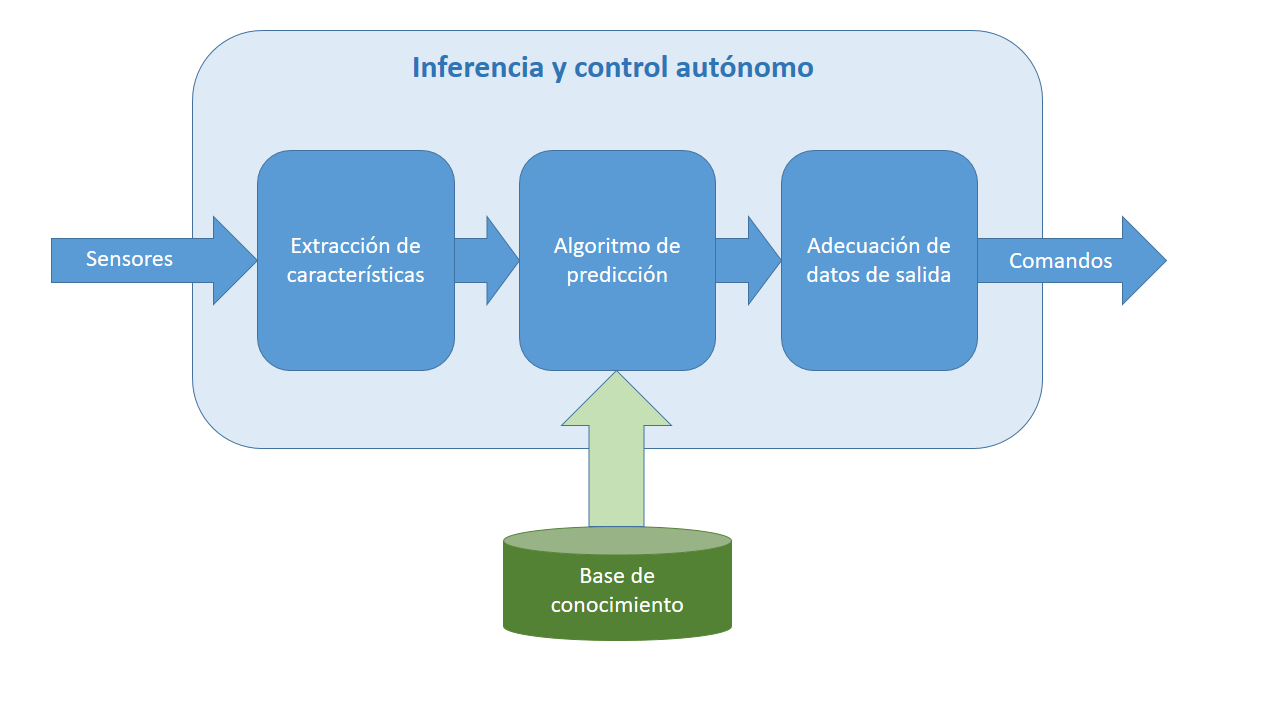
\includegraphics[width=0.39\textwidth]{../img/inferencia}
      \end{figure}
  
  \end{frame}

\begin{frame}{Objetivo General}
    Diseñar un sistema de aprendizaje \emph{“fin a fin”} capaz de generar de comandos de 
control de vehículos domésticos basado en visión artificial y \alert{redes neuronales 
convolucionales} para facilitar el diseño e implementación de sistemas de conducción autónoma.
\end{frame}

\begin{frame}{Objetivos Específicos}
    \begin{itemize}

        \item Estudiar los aspectos concernientes a los sistemas de conducción autónoma y sistemas de aprendizaje.
        \item Analizar los requerimientos.
        \item Diseñar la arquitectura del sistema.
        \item Diseñar el subsistema de control y actuación.
        \item Diseñar el subsistema de adquisición de datos y entrenamiento.
        \item Diseñar el subsistema de inferencia y control autónomo.
        \item Analizar los resultados del entrenamiento e implementación.
        \item Realizar pruebas de rendimiento y análisis comparativos.
    
    \end{itemize}
\end{frame}


\section{Fundamento Teórico}

\begin{frame}{Sistemas de Conducción Autónoma}
    Un sistema de conducción autónoma tiene la capacidad de operar un vehículo 
    de forma completamente autónoma.
    \begin{figure}[!h] 
        \centering
        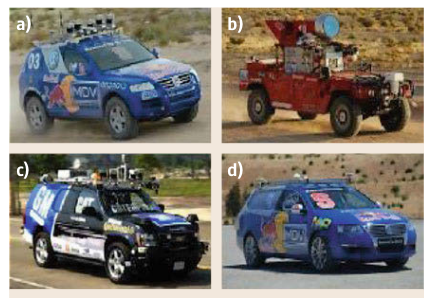
\includegraphics[width=0.45\textwidth]{../img/darpa}
        \caption[Vehículos del \textit{Grand Challenge}]{Vehículos del \textit{Grand Challenge} de 2005: (a) Stanley (1er lugar), (b) Sandstorm (2do lugar). Vehículos del \textit{Urban Challenge} de 2007: (c) Boss (1er lugar) (d) Junior (2do lugar). Fuente: \cite{wikipedia_2018} }
    \end{figure}
\end{frame}

\begin{frame}{Niveles de Autonomía SAE}
    Se han definido distintos niveles de autonomía por parte de la Sociedad de Ingenieros de Automoción (SAE).
    \begin{figure}[!h] 
        \centering
        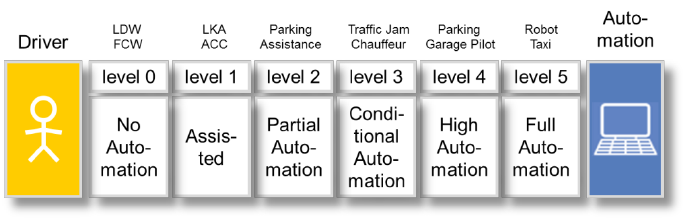
\includegraphics[width=0.75\textwidth]{../img/levels}
        \caption[Niveles de automatización SAE]{Niveles de automatización en la conducción según SAE. 
        Fuente: \href{https://www.researchgate.net/figure/Terms-related-to-automated-driving-according-to-SAE-and-VDA_fig1_273883061}{researchgate} }
\end{figure}
\end{frame}

\begin{frame}{Visión Artificial}
    \begin{columns}
        \begin{column}{0.5\textwidth}
            Es un campo de las ciencias de la computación que intenta reproducir las capacidades de una persona para entender imágenes.
            Aplicaciones:
            \begin{itemize}
                \item \small{Reconocimiento óptico de caracteres (OCR).}
                \item Inspección automática.
                \item Ventas.
                \item Reconstrucción de modelos en 3D (fotogrametría).
                \item Imagenología médica.
                \item Seguridad automotriz.
                \item Seguridad y vigilancia.
            \end{itemize}
        \end{column}
        \begin{column}{0.5\textwidth}
            \begin{figure}[!h] 
                \centering
                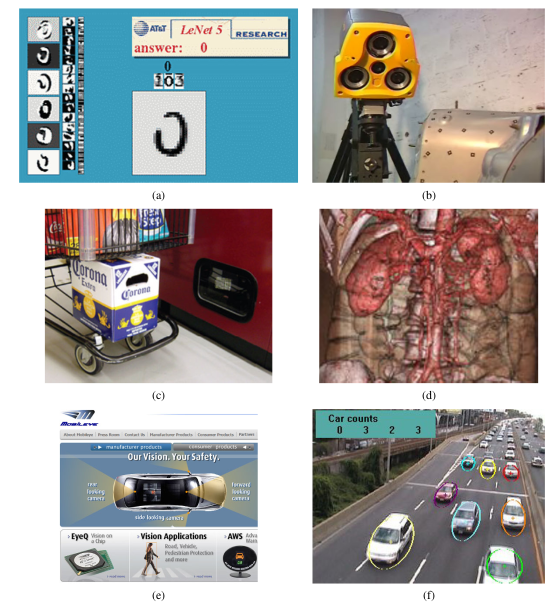
\includegraphics[width=0.95\textwidth]{../img/cvision}
                \caption[Algunas aplicaciones de la visión artificial]{Algunas aplicaciones de la visión artificial. Fuente: \cite{Szeliski2011} }
            \end{figure}
        \end{column}
    \end{columns}
    
\end{frame}

% \begin{frame}{Visión Artificial}
%     \begin{figure}[!h] 
%         \centering
%         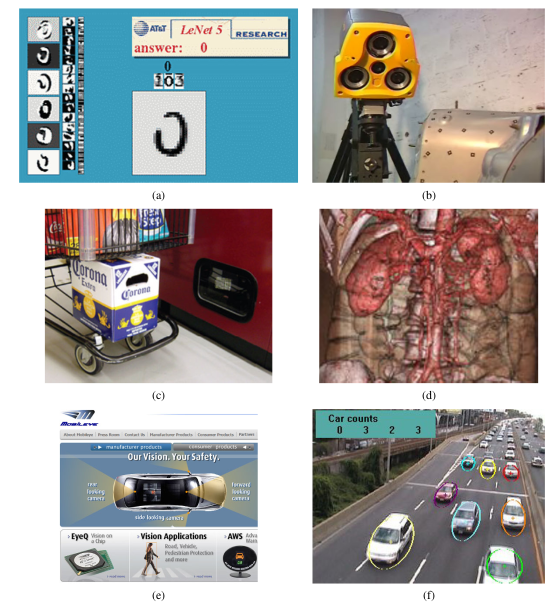
\includegraphics[width=0.55\textwidth]{../img/cvision}
%         \caption[Algunas aplicaciones de la visión artificial]{Algunas aplicaciones de la visión artificial. Fuente: \cite{Szeliski2011} }
%     \end{figure}
% \end{frame}

\subsection{Redes Neuronales Artificiales}
\begin{frame}{Redes Neuronales Artificiales}
    Las redes neuronales artificiales son un modelo matemático de cómputo muy útiles en la aproximación de funciones y reconocimiento de patrones.

    \begin{figure}[!h] 
        \centering
        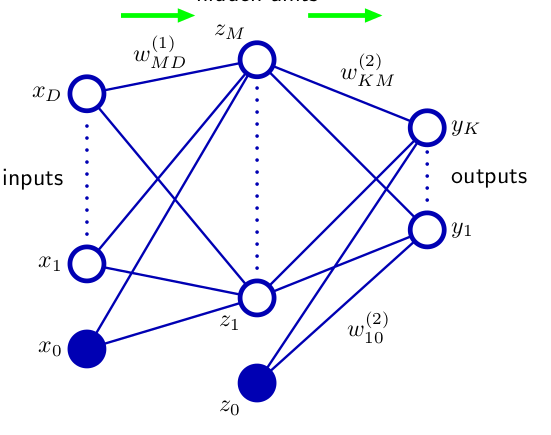
\includegraphics[width=0.65\textwidth]{../img/reddoscapas}
        \caption[Diagrama de una red neuronal de dos capas]{Diagrama de la red neuronal de dos capas. Fuente: \cite{Bishop2006} }
        \label{fig:reddoscapas}
    \end{figure}

\end{frame}

\begin{frame}{Redes Neuronales Artificiales}
    \begin{figure}[!h] 
        \centering
        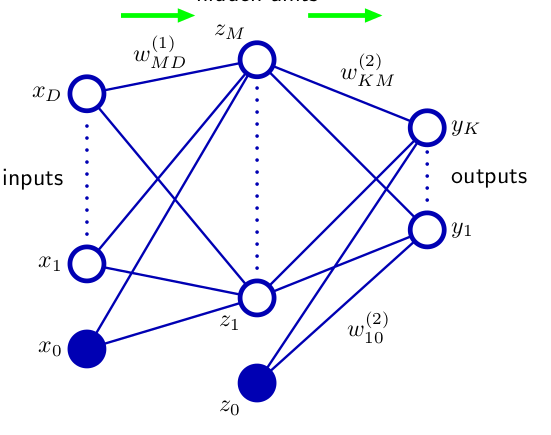
\includegraphics[width=0.50\textwidth]{../img/reddoscapas}
        \label{fig:reddoscapas}
    \end{figure}
    Ecuación correspondiente:
    \begin{equation}\label{eq:reddoscapas}
        y_k(\mathbf{x}, \mathbf{W}) = \sigma \left( \sum_{j=1}^M w_{kj}^{(2)} h \left( \sum_{i=1}^D w_{ji}^{(1)} x_i + w_{j0}^{(1)} \right) + w_{k0}^{(2)} \right)
    \end{equation}
\end{frame}

\begin{frame}{Función de Costo}
    La función de costo permite definir el rendimiento de la red con respecto a las predicciones esperadas a la salida.

    Dado un conjunto de entrenamiento compuesto por un conjunto de vectores 
        de entrada $\{\mathbf{x}_n \}$, donde $n = 1, \ldots , N$, junto con un conjunto de vectores objetivo $\{\mathbf{t}_n \}$
        el objetivo es \alert{minimizar la función}:

        \begin{equation}\label{eq:error}
            E(\mathbf{w}) = \frac{1}{2} \sum_{n=1}^N \{y(\mathbf{x}_n, \mathbf{w}) - t_n\}^2
        \end{equation}

\end{frame}

\begin{frame}{Descenso de Gradiente}
    \begin{figure}[!h] 
        \centering
        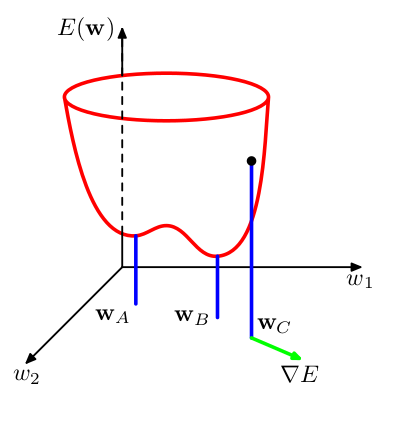
\includegraphics[width=0.55\textwidth]{../img/gradsup}
        \caption[Visualización de la función de error]{Visualización de la función de error $E(\mathbf{w})$ como una superficie. El punto $\mathbf{w}_A$ es un mínimo local y el punto $\mathbf{w}_B$ es el mínimo global. Fuente: \cite{Bishop2006} }
    \end{figure}
    
\end{frame}

% \begin{frame}{Funciones de Activación}
%     Las funciones de activación contibuyen en la naturaleza no lineal de las 
%     capas ocultas de la red. 

%     Deben contribuir con la calidad de las representaciones internas de la red así como 
%     también poseer un buen comportamiento en sus gradientes para el entrenamiento.

% \end{frame}

\begin{frame}{Redes Neuronales Convolucionales}
    Las redes convolucionales usan la función de convolución para procesar 
    la información en cada capa oculta. 

    La operación de convolución para señales digitales se define de la siguiente manera:
    \begin{equation}
        s(t) = (x \ast w)(t) = \sum_{\tau=-\infty}^{\infty}x(\tau)w(t-\tau)
    \end{equation}
    Para el caso de una imagen en 2D, la convolución se define como:
    \begin{equation}
        S(i,j)=(K\ast I)(i,j) = \sum_{m} \sum_{n} I(i-m,j-n)K(m,n)
    \end{equation}

\end{frame}

\begin{frame}{Redes Neuronales Convolucionales}
    La operación de convolución se puede aplicar a imágenes (matrices multidimensionales):

    \begin{figure}[!h] 
        \centering
        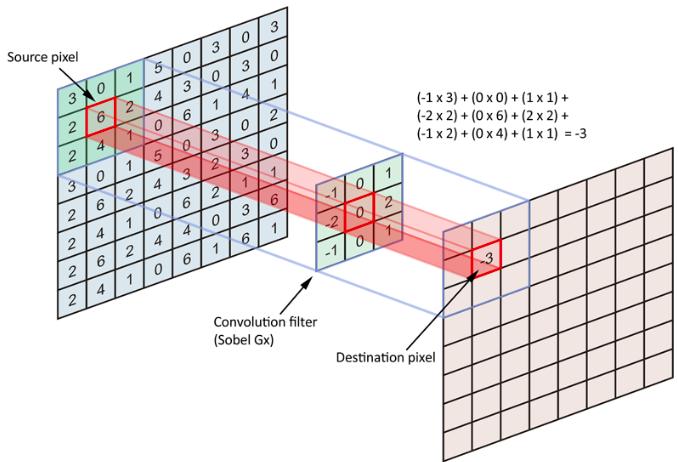
\includegraphics[width=0.60\textwidth]{../img/convolucion}
        \caption[Visualización de la operación de convolución sobre una imagen digital]{Visualización de la operación de convolución sobre una imagen digital. Fuente: \cite{cornelisse_2018} }
    \end{figure}
\end{frame}

\begin{frame}{Sistemas de Aprendizaje Fin a Fin}
    Los sistemas de aprendizaje fin a fin son modelos de aprendizaje que tratan ciertos problemas 
    \alert{de manera conjunta} en lugar de separarlos en módulos o etapas de procesamiento.

    Las representaciones internas de un sistema fin a fin se encargan de abstraer el conocimiento en 
    base a la experiencia previa presentada en el conjunto de datos y no necesita de un experto que atienda 
    el desarrollo de las mismas.

\end{frame}

\section*{Ingeniería del proyecto}

\begin{frame}{Arquitectura del Sistema}
    \begin{figure}[!h] 
        \centering
        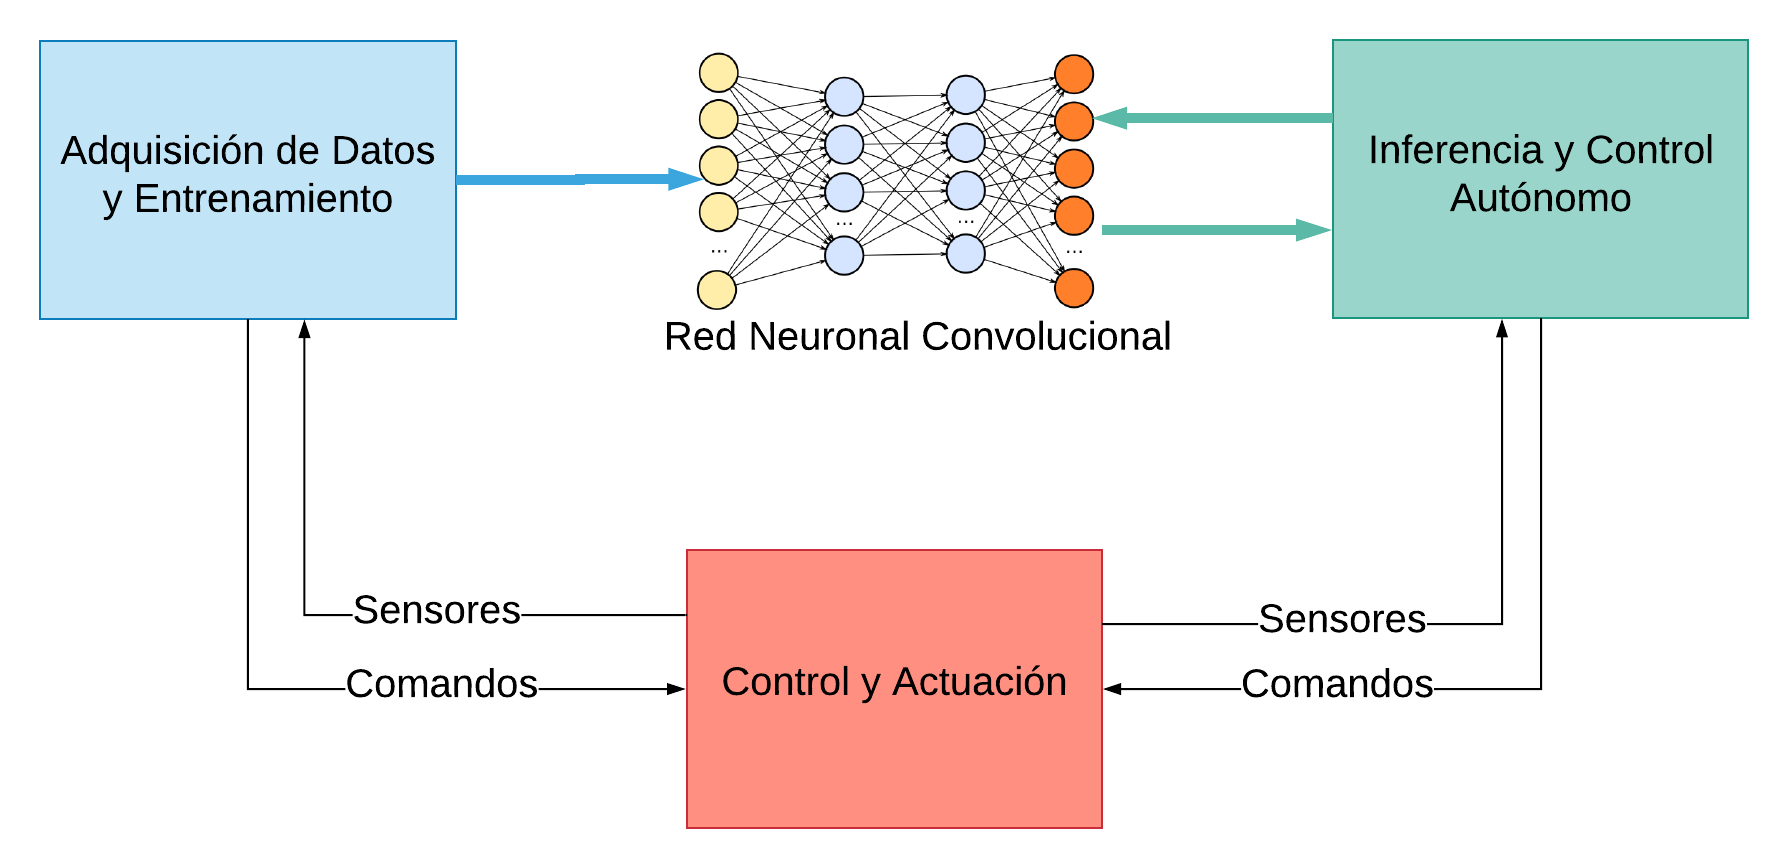
\includegraphics[width=0.85\textwidth]{../img/arquitectura}
        \end{figure}
\end{frame}

\section{Subsistema de Control y Actuación}
\begin{frame}{Esquema}
    \begin{figure}[!h] 
        \centering
        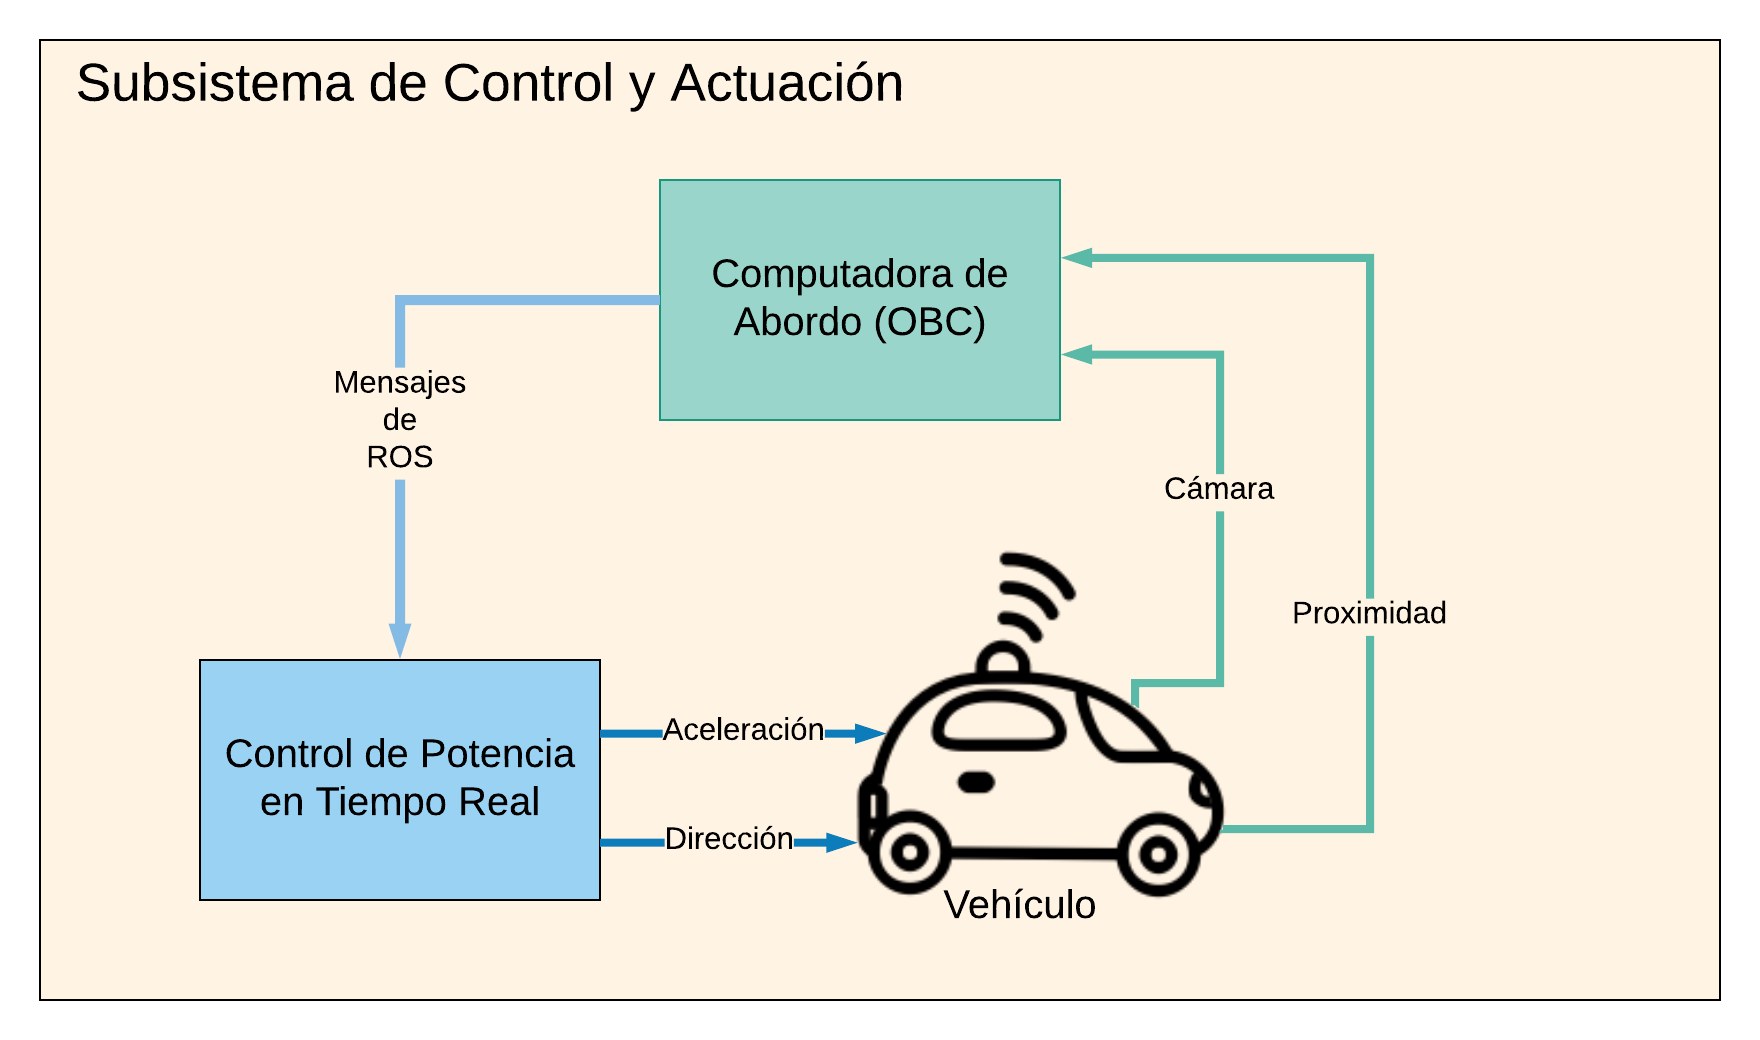
\includegraphics[width=0.85\textwidth]{../img/control_esq}
        \end{figure}
\end{frame}

% \begin{frame}{Tareas}
%     Este subsistema cuenta con módulos que tienen tres principales responsabilidades.
    
%     \begin{itemize}
%         \item Ejecutar un control de tiempo real en los actuadores disponibles para la locomoción del vehículo a través de un sistema embebido.
%         \item Brindar una plataforma para la adquisición de los datos de los sensores (la cámara y el sensor de proximidad).
%         \item Brindar una plataforma de desarrollo para el control autónomo del vehículo mediante ROS.
%     \end{itemize}  
% \end{frame}

\begin{frame}{Módulo de potencia en tiempo real}
    Se encarga del control de los actuadores mediante un sistema embebido 
    que tiene capacidades de tiempo real.

    \begin{figure}[!h] 
        \centering
        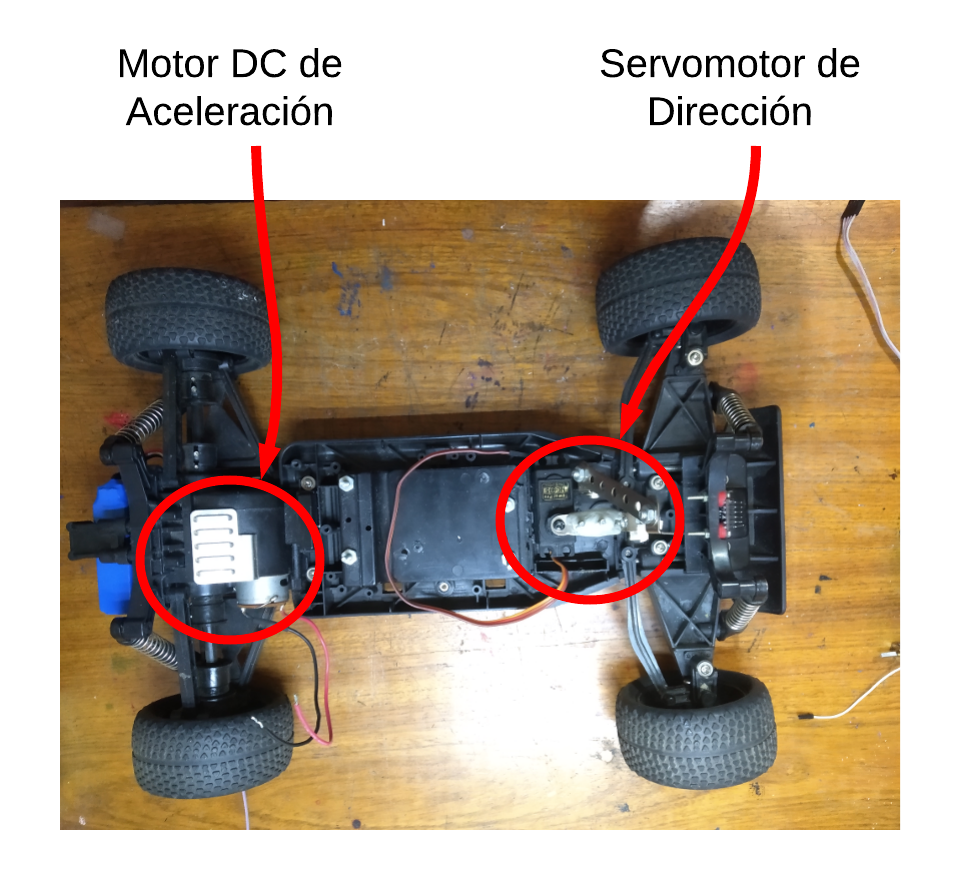
\includegraphics[width=0.45\textwidth]{../img/actuadores}
        \end{figure}
\end{frame}

\begin{frame}{Módulo de potencia en tiempo real}
    Se encarga del control de los actuadores mediante un sistema embebido 
    que tiene capacidades de tiempo real.

    \begin{figure}[!h] 
        \centering
        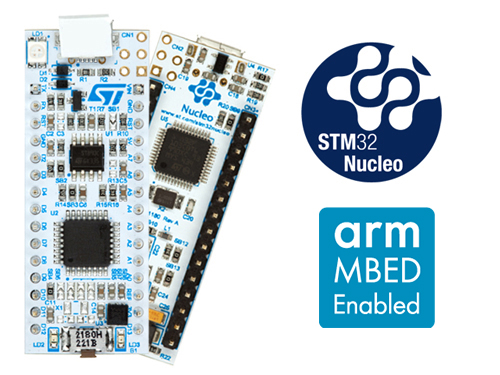
\includegraphics[width=0.45\textwidth]{../img/nucleo}
        \caption[Placa de desarrollo Nucleof303k8 de ST Microelectronics]{Placa de desarrollo Nucleof303k8 de ST Microelectronics. Fuente: \cite{nucleof303} }
        \end{figure}
\end{frame}


\begin{frame}{Módulo de la computadora de abordo (OBC)}
    La OBC se encarga del control de alto nivel del vehículo. Sus principales tareas son:
    \begin{itemize}
        \item Recepción de comandos de control remoto.
        \item Comunicación de los nodos de procesamiento del sistema.
        \item Envío de comandos de control al módulo de tiempo real.
    \end{itemize}
\end{frame}

\begin{frame}{Módulo de la computadora de abordo (OBC)}
    \begin{figure}[!h] 
        \centering
        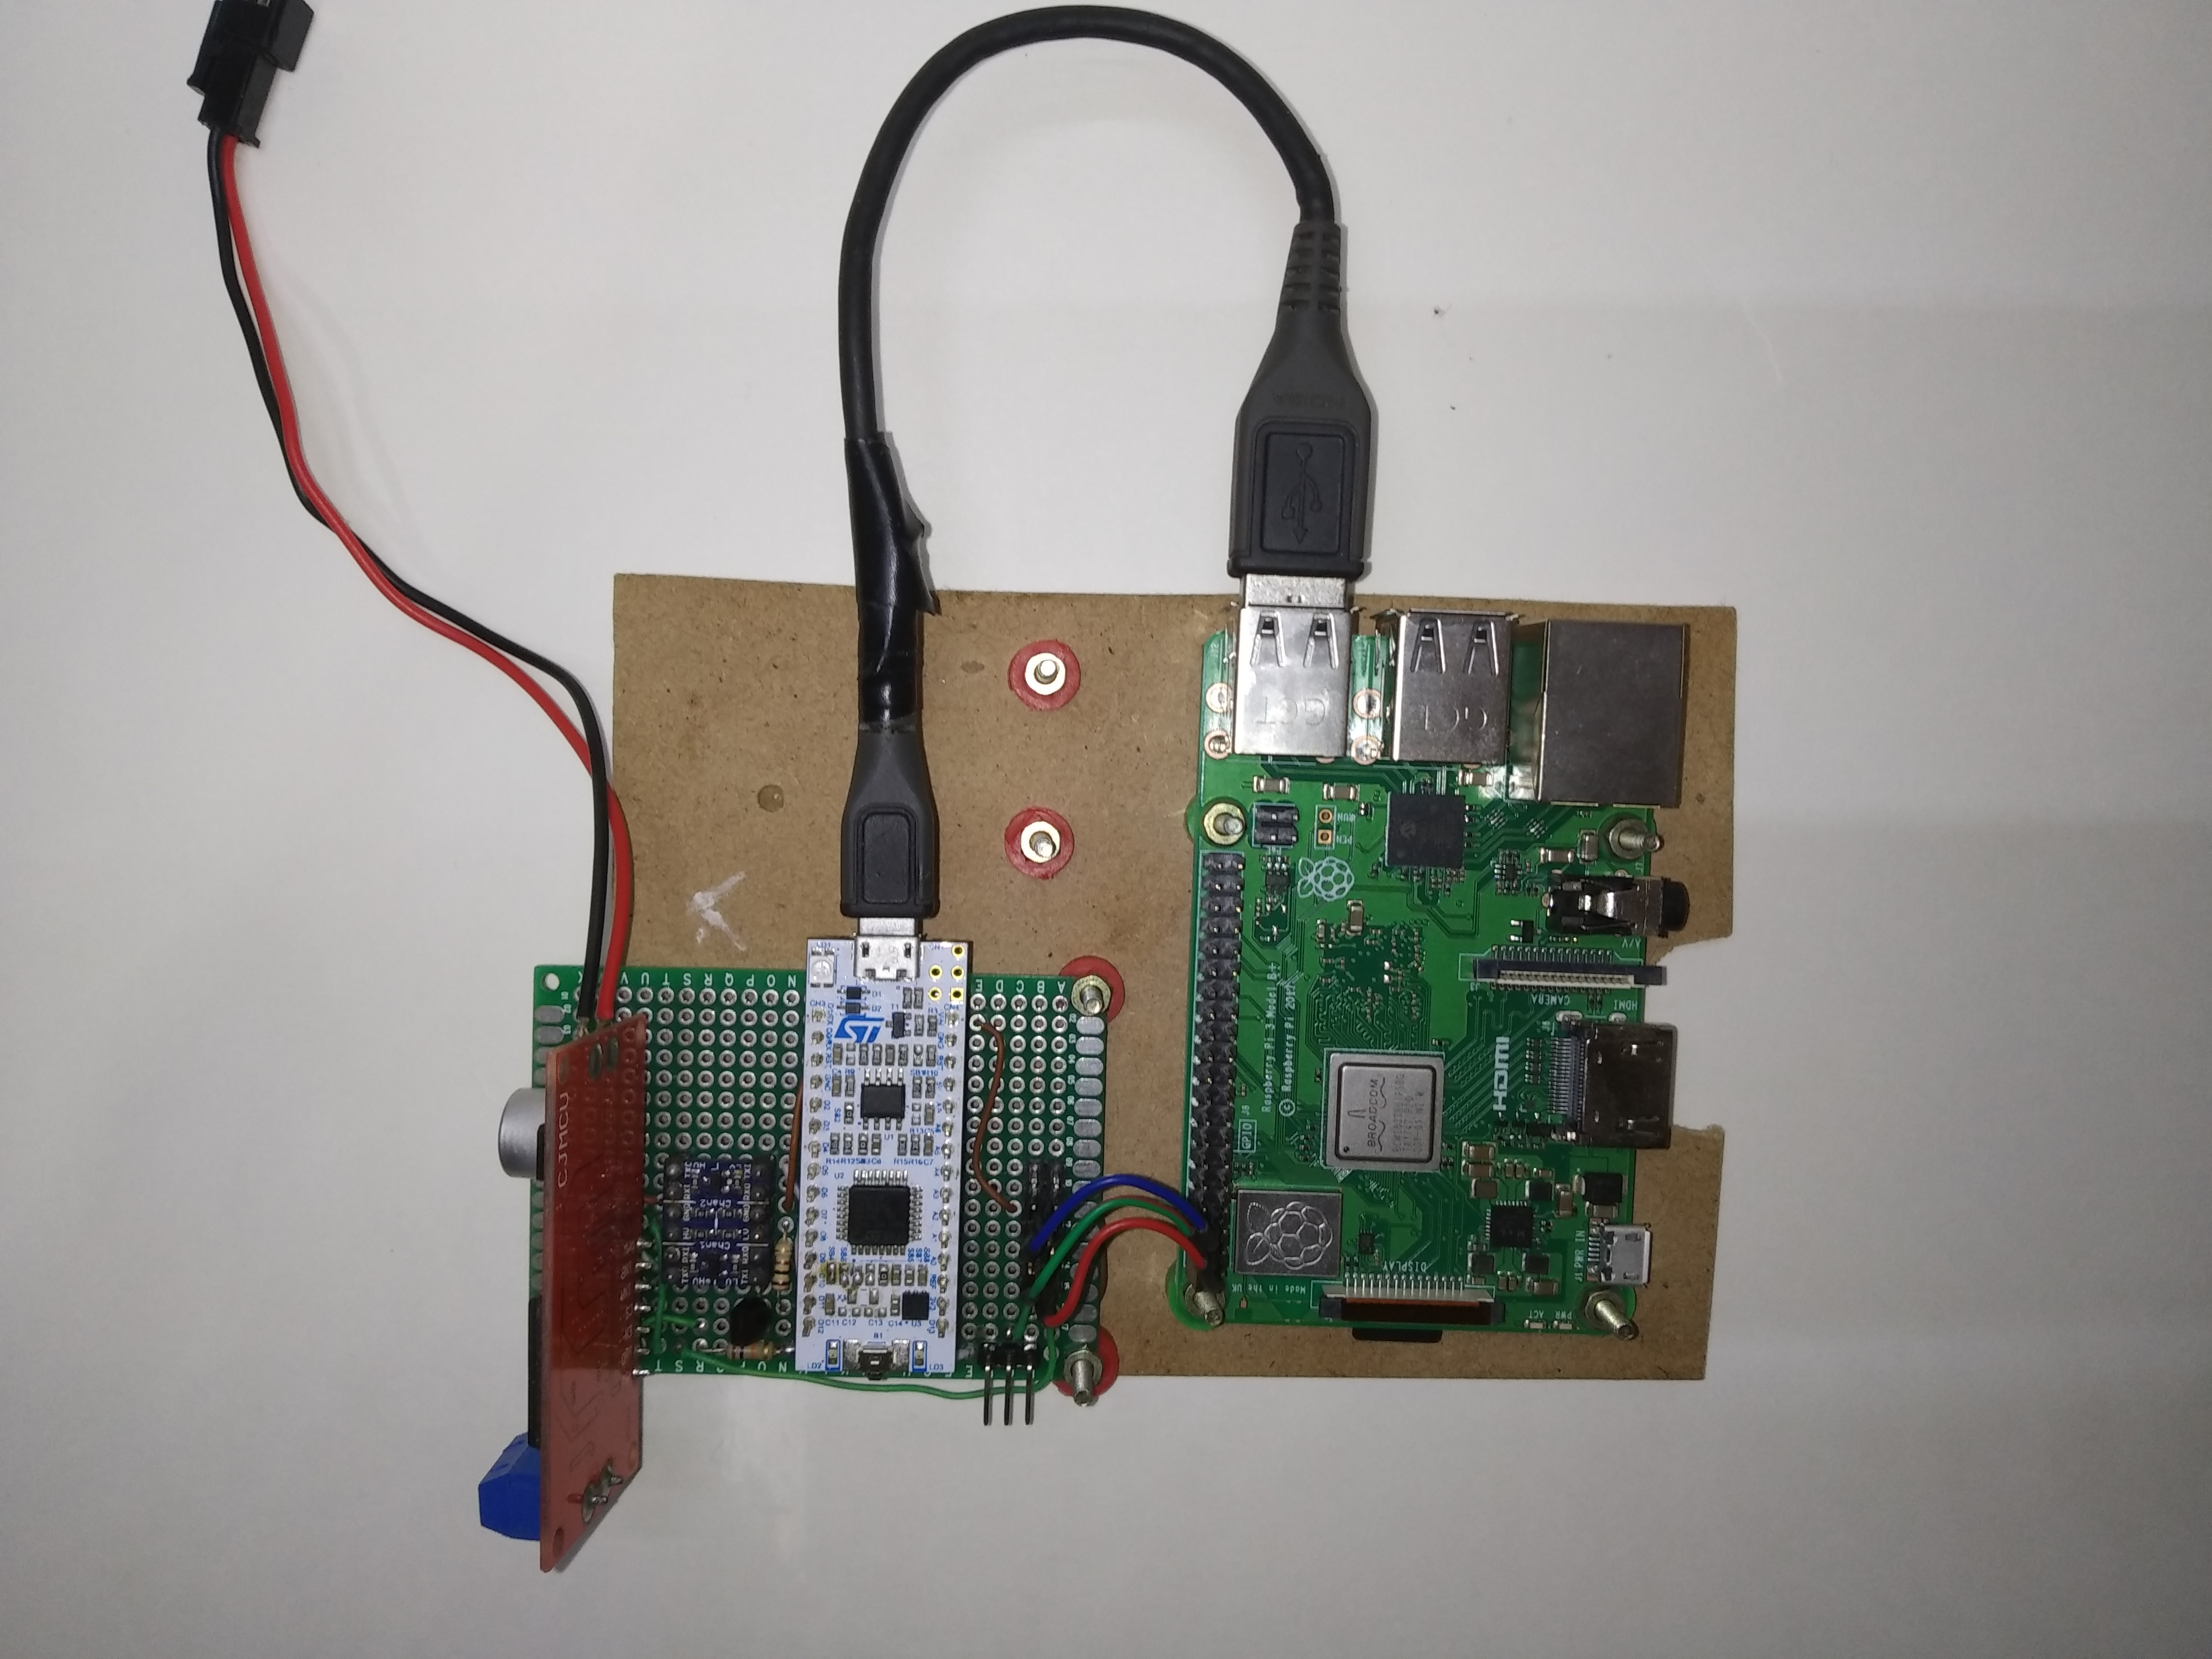
\includegraphics[width=0.55\textwidth]{../img/obc}
        \caption[Fotografía de la OBC]{Fotografía de la OBC. Fuente: Elaboración propia. }
    \end{figure}
\end{frame}

\begin{frame}{Módulo de la computadora de abordo (OBC)}
    \begin{figure}[!h] 
        \centering
        \includegraphics[width=0.55\textwidth]{../img/carro}
        \caption[Fotografía del prototipo]{Fotografía del prototipo. Fuente: Elaboración propia. }
        \end{figure}
\end{frame}

\begin{frame}{Módulo de la computadora de abordo (OBC)}
    \begin{figure}[!h] 
        \centering
        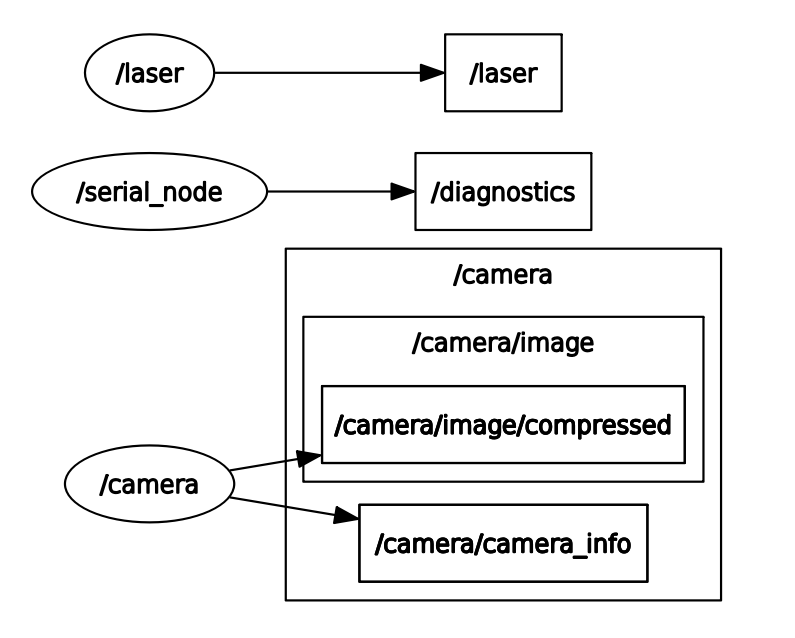
\includegraphics[width=0.55\textwidth]{../img/nodosobc}
        \caption[Interacción de los nodos en la OBC]{Interacción de los nodos en la OBC. Fuente: Elaboración propia. }
    
    \end{figure}
\end{frame}


\section{Subsistema de Adquisición de Datos y Entrenamiento}

\begin{frame}{Esquema}
    \begin{figure}[!h] 
        \centering
        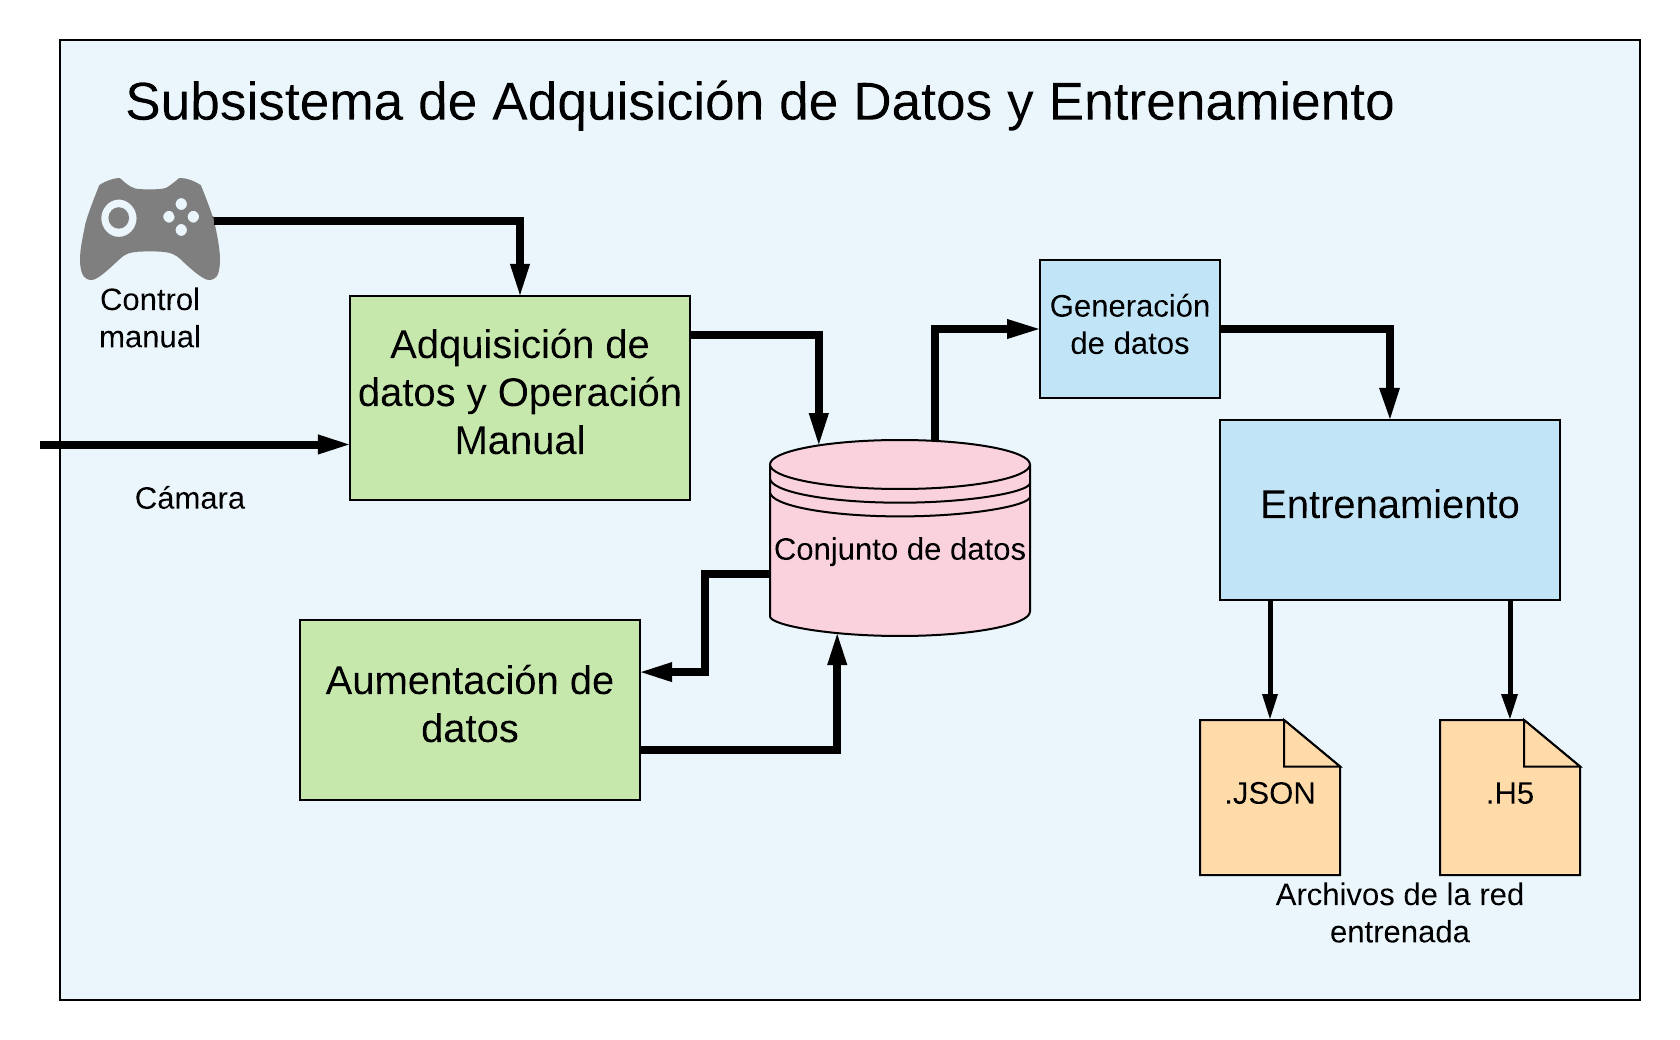
\includegraphics[width=0.85\textwidth]{../img/daq_esq}
        \end{figure}
\end{frame}

% \begin{frame}{Tareas}
%     \begin{itemize}
%         \item Generar un conjunto de datos o \textit{dataset} para el entrenamiento y validación de la red neuronal.
%         \item Entrenar una red neuronal a partir del conjunto de datos y ciertos parámetros previamente definidos.
%     \end{itemize}
% \end{frame}

\begin{frame}{Módulo de Adquisición de Datos y Operación Manual}
    Se realiza la adquisición de datos mientras se opera el vehículo manualmente.
    
    Este modo de funcionamiento permite almacenar datos para el entrenamiento.

    \begin{figure}[!h] 
        \centering
        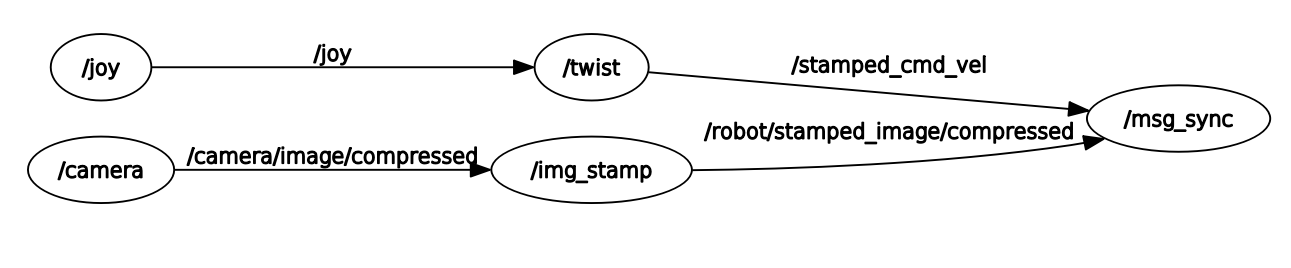
\includegraphics[width=0.95\textwidth]{../img/nodosdaq}
        \end{figure}
    
\end{frame}


\begin{frame}{Módulo de Adquisición de Datos y Operación Manual}
    \begin{figure}[!h] 
        \centering
        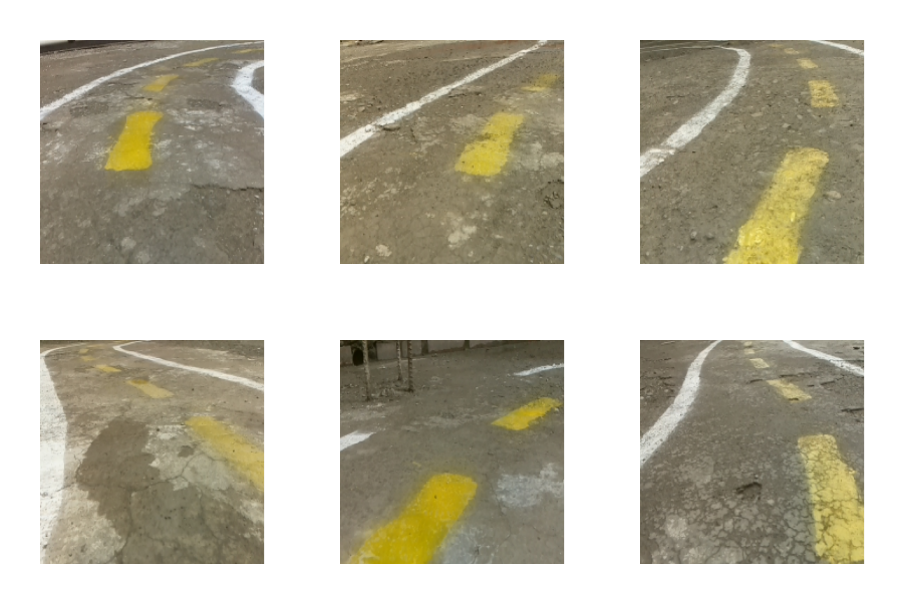
\includegraphics[width=0.75\textwidth]{../img/fotosejemplo}
        \caption[Imágenes capturadas por la cámara en una sesión de entrenamiento]{Imágenes capturadas por la cámara en una sesión de entrenamiento. Fuente: Elaboración propia. }
    \end{figure}
    
\end{frame}

\begin{frame}{Módulo de Aumentación de Datos}
    Una de las desventajas de las redes neuronales es que se necesita una 
    cantidad sustancialmente superior de datos que en otros algoritmos de visión 
    artificial.

    Por su parte, la obtención del conjunto de datos es uno de los procesos más costosos en tiempo 
    y recursos en un sistema de aprendizaje.

\end{frame}

\begin{frame}{Módulo de Aumentación de Datos}
    \begin{table}[!h]
        \centering
        \resizebox{0.65\textwidth}{!}{%
        \begin{tabular}{@{}|c|c|@{}}
        \toprule
        \textbf{Transformación} & \textbf{Descripción}                                                                                                      \\ \midrule
        Rotación                & \begin{tabular}[c]{@{}c@{}}Rotación de la imagen en un ángulo \\ aleatorio entre -20 y 20 grados.\end{tabular}                   \\ \midrule
        Desplazamiento Vertical & \begin{tabular}[c]{@{}c@{}}Desplazamiento de la imagen de forma \\ vertical un valor aleatorio entre \\ 0 y 20 \%.\end{tabular} \\ \midrule
        Espejo Horizontal       & \begin{tabular}[c]{@{}c@{}}Espejado de la imagen \\ horizontalmente de forma aleatoria.\end{tabular}                      \\ \bottomrule
        \end{tabular}%
        }
        \caption[Transformaciones realizadas en la aumentación de datos.]{Transformaciones realizadas en la aumentación de datos. Fuente: Elaboración propia.}
    \end{table}

\end{frame}

\begin{frame}{Módulo de Aumentación de Datos}
    \begin{figure}[!h] 
        \centering
        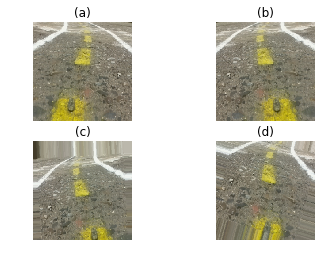
\includegraphics[width=0.65\textwidth]{../img/aumentacion}
        \caption[Ejemplos de aumentación de datos]{Ejemplos del proceso de aumentación de datos: (a) imagen original, 
        imagen espejada horizontalmente, (c) imagen desplazada verticalmente, (d) imagen rotada. Fuente: Elaboración propia. }
    \end{figure}

\end{frame}

% \begin{frame}{Módulo de Generación de Datos}
%     Este módulo genera conjuntos pequeños de imágenes que se cargan a la memoria 
%     de manera progresiva para el entrenamiento debido a que no se puede cargar todo el 
%     conjunto de entrenamiento de una sola vez.
% \end{frame}

\begin{frame}{Módulo de Entrenamiento}
    Este módulo realiza las siguientes tareas:

    \begin{itemize}
        \item Cargar el dataset y el modelo de la red.
        \item Definir hiperparámetros.
        \item Ejecutar y monitorear el entrenamiento.
        \item Salvaguardar parámetros.
        \item Generar reportes del entrenamiento.
    \end{itemize}
\end{frame}

\begin{frame}{Módulo de Entrenamiento}
    El módulo tiene como salida dos archivos:

    \begin{itemize}
        \item \textbf{Arquitectura de la red neuronal:} Se almacena la información acerca de la arquitectura de la red en un archivo con formato \emph{JSON} donde se puede encontrar la información acerca de las dimensiones de las capas ocultas, cantidad de unidades por capa y dimensiones de cada unidad en la red.
        \item \textbf{Pesos entrenados de la red neuronal:} Se almacena también los valores de todos los parámetros o pesos de la red neuronal, resultado del entrenamiento. Estos valores están almacenados en un archivo con extensión \emph{H5}. 
    \end{itemize}

\end{frame}


\section{Subsistema de Inferencia y control autónomo}
\begin{frame}{Esquema}
    \begin{figure}[!h] 
        \centering
        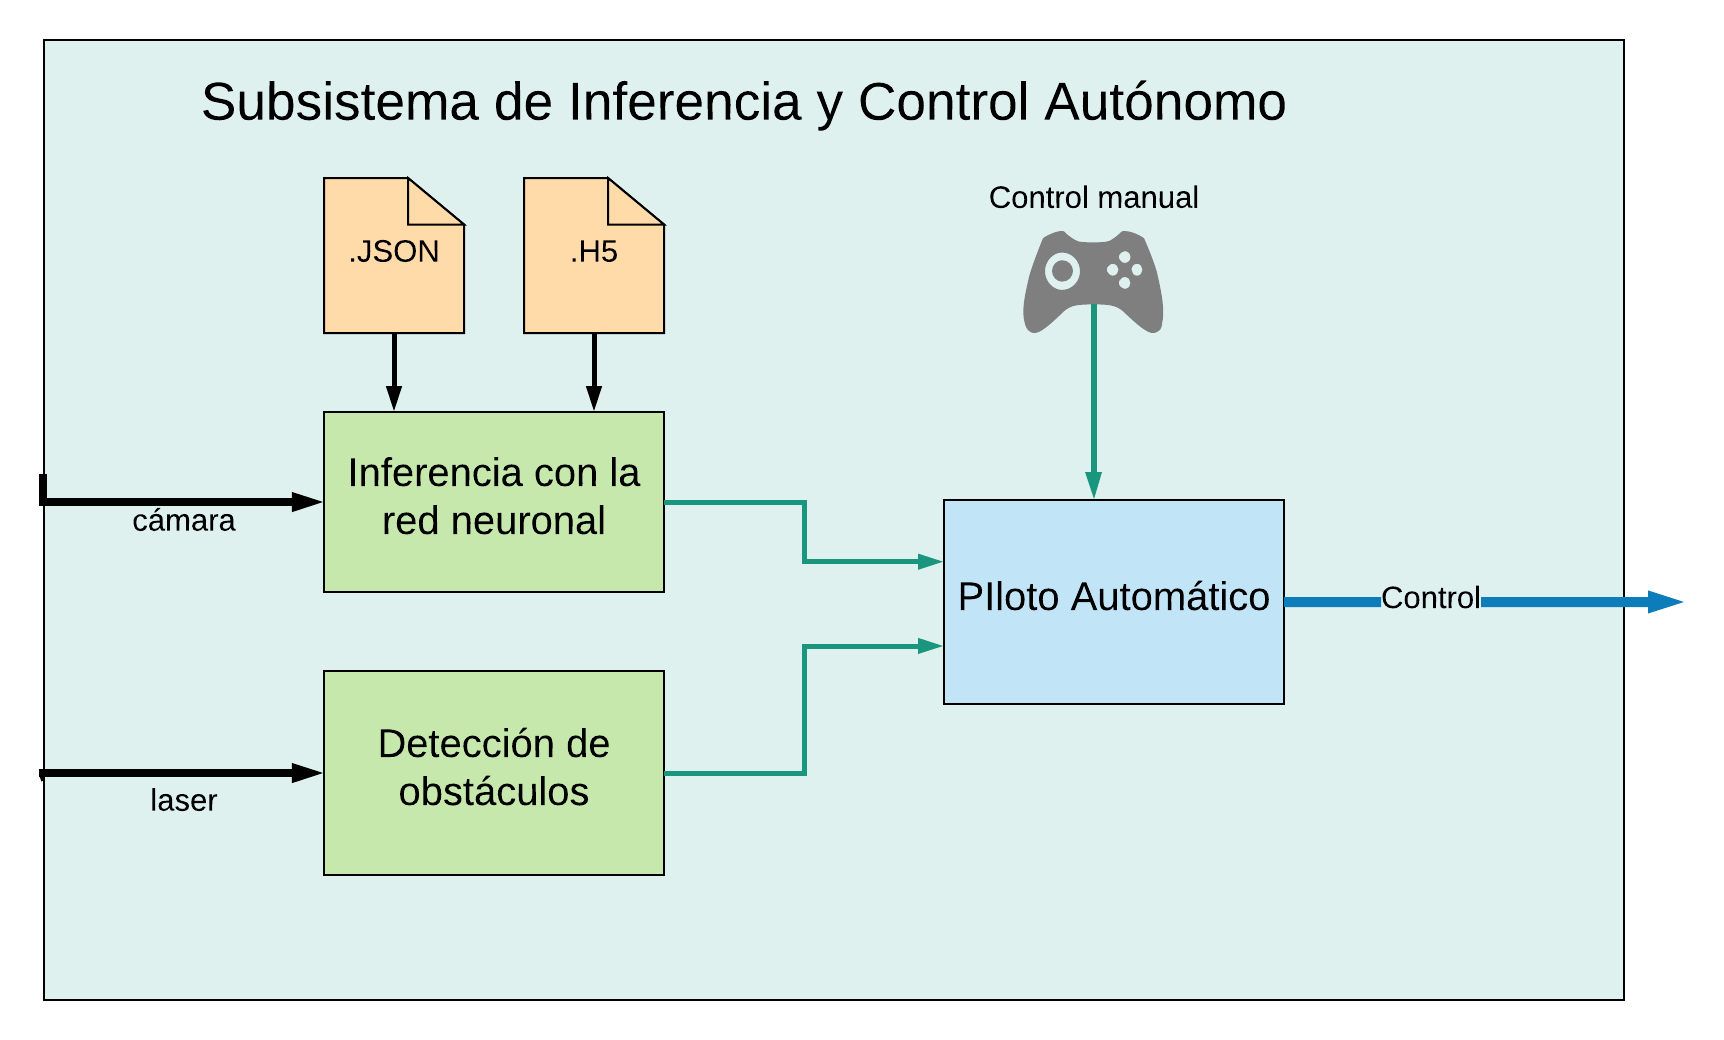
\includegraphics[width=0.85\textwidth]{../img/inferencia_esq}
        \end{figure}
\end{frame}

% \begin{frame}{Tareas}
%     El subsistema debe cumplir las siguientes tareas:
%     \begin{itemize}
%         \item Cargar y ejecutar el modelo de predicción implementado en la red neuronal entrenada en el subsistema de adquisición de datos y entrenamiento para la generación de comandos de dirección del vehículo.
%         \item Ejecutar un algoritmo de control para la aceleración basado en la detección de obstáculos presentes frente al vehículo.
%         \item Ejecutar un algoritmo de arbitraje que combine ambos sistemas de control en conjunto con un control manual de respaldo que será referido como el \textit{piloto automático}.
%     \end{itemize} 
% \end{frame}

\begin{frame}{Módulo de Inferencia Neuronal}
    Este módulo tiene la tarea de ejecutar la tarea de predicción del comando de control de dirección con la red neuronal 
    entrenada por el módulo de entrenamiento del subsistema de adquisición de datos y entrenamiento.
    \begin{figure}[!h] 
        \centering
        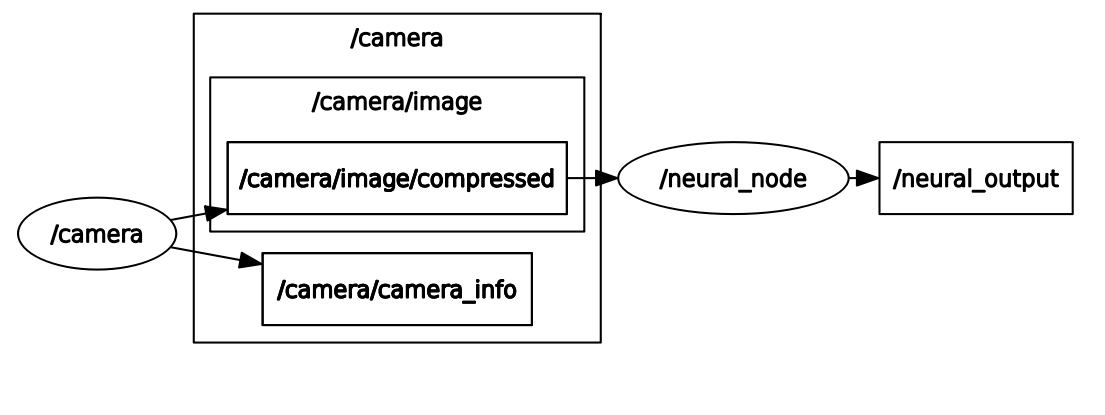
\includegraphics[width=0.95\textwidth]{../img/nodosneural}
        \end{figure}
\end{frame}


\begin{frame}{Módulo de detección de obstáculos}
    El módulo de detección de obstáculos tiene la finalidad de controlar la aceleración del vehículo basado en la 
    presencia de obstáculos físicos frente al mismo. Se basa en las mediciones de proximidad realizadas por el 
    sensor de proximidad montado en frente del vehículo. 

    \begin{figure}[!h] 
        \centering
        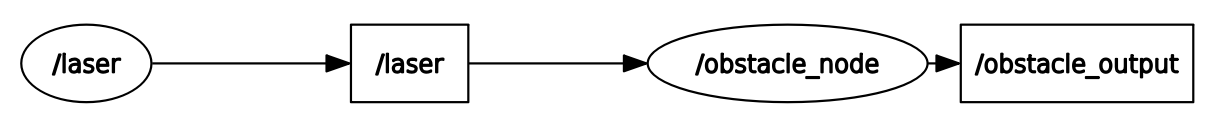
\includegraphics[width=0.95\textwidth]{../img/nodosobs}
        \end{figure}
\end{frame}


\begin{frame}{Módulo del piloto automático}
    Este módulo se encarga de arbitrar los comandos de control provenientes de las distintas fuentes utilizadas en el sistema. Se 
    suscribe a cada tópico correspondiente y redirecciona los mensajes para el control del vehículo mediante mensajes.

    \begin{figure}[!ht] 
        \centering
        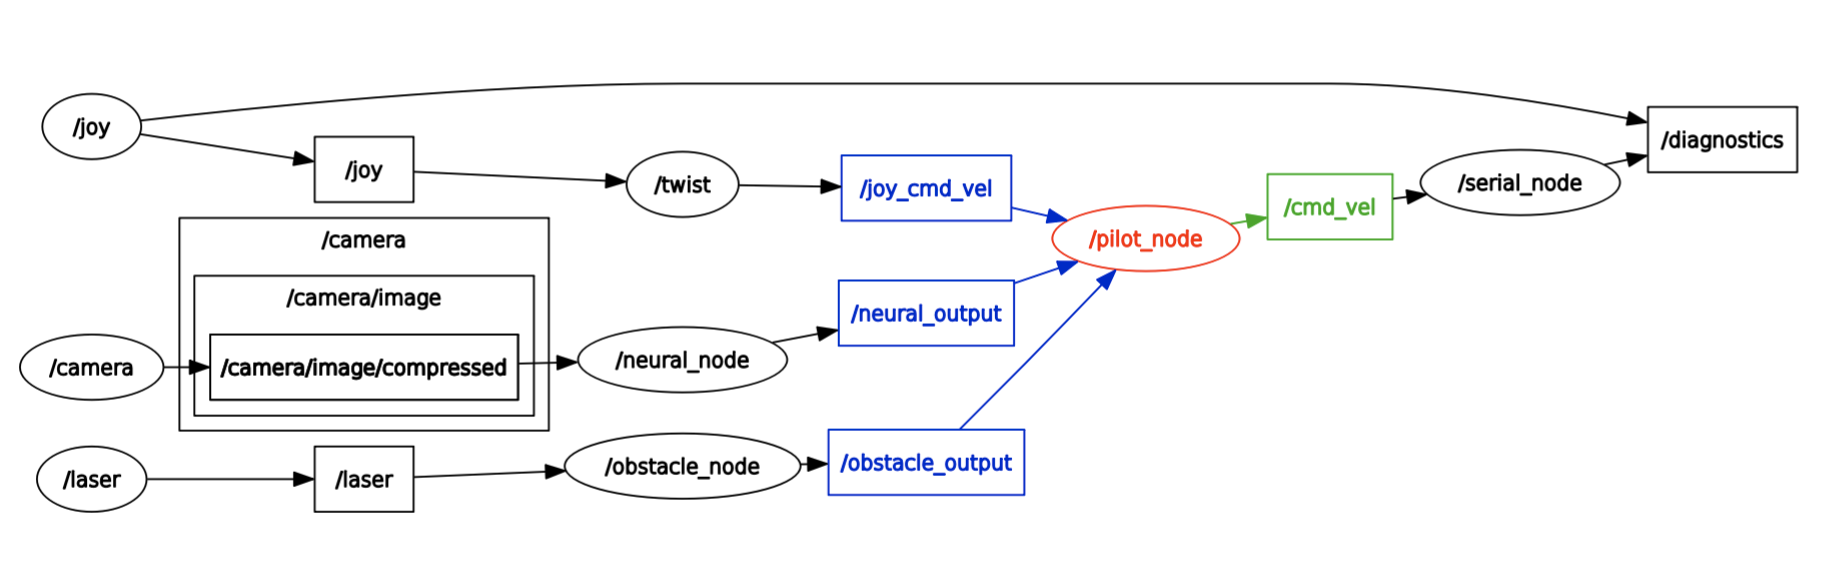
\includegraphics[width=\textwidth]{../img/nodesauto}
        \end{figure}

\end{frame}

\section*{Arquitectura de la Red Neuronal}

% \begin{frame}{Capas Convolucionales}
%     \begin{figure}[!ht] 
%         \centering
%         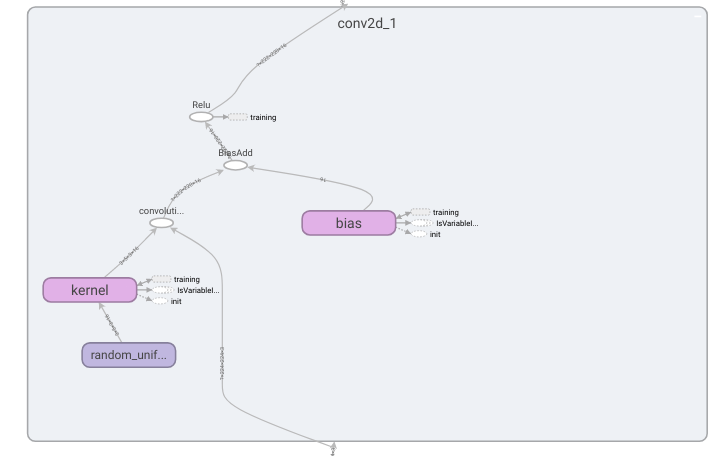
\includegraphics[width=0.85\textwidth]{../img/convlayer}
%     \end{figure}
% \end{frame}

% \begin{frame}{Pooling}
%     \begin{figure}[!ht] 
%         \centering
%         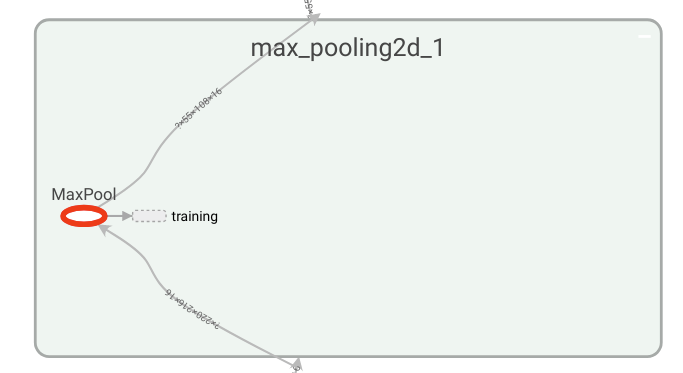
\includegraphics[width=0.85\textwidth]{../img/maxpooltf}
%     \end{figure}
% \end{frame}

% \begin{frame}{Capas Densamente Conectadas}
%     \begin{figure}[!ht] 
%         \centering
%         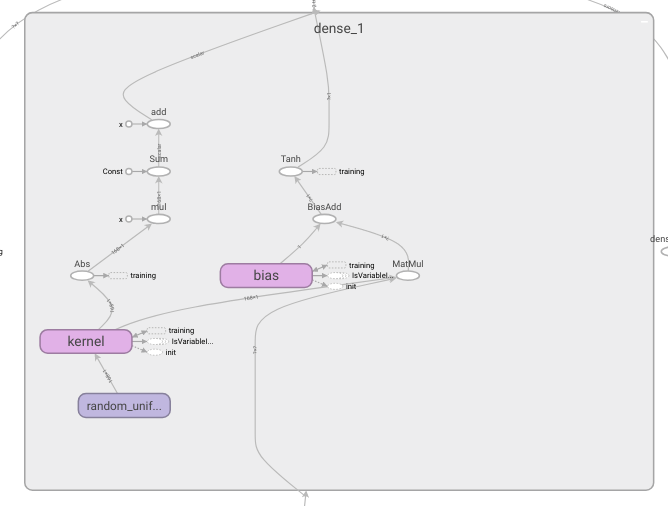
\includegraphics[width=0.85\textwidth]{../img/densetf}
%     \end{figure}
% \end{frame}

\begin{frame}{Funciones de Activación - RELU}
    \begin{equation}\label{eq:relu}
        g(x) = max\{0,x\}
    \end{equation}

    \begin{figure}[!h] 
        \centering
        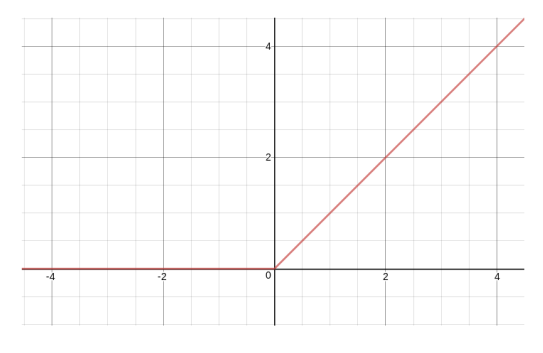
\includegraphics[width=0.75\textwidth]{../img/relu}
        \caption[Gráfico de la función ReLU]{Gráfico de la función ReLU. Fuente: \cite{wang_2016} }
    \end{figure}
\end{frame}

\begin{frame}{Funciones de Activación - Tanh}
    \begin{equation}\label{eq:tanh}
        tanh(x) = \frac{e^x - e^{-x}}{e^x + e^{-x}}
    \end{equation}

    \begin{figure}[!h] 
        \centering
        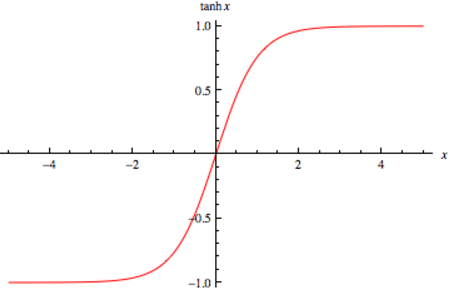
\includegraphics[width=0.75\textwidth]{../img/tanh}
        \caption[Gráfico de la función tangente hiperbólica]{Gráfico de la función tangente hiperbólica $tanh(x) = \frac{e^x - e^{-x}}{e^x + e^{-x}}$. Fuente: \cite{wang_2016} }
                \end{figure}
\end{frame}

\begin{frame}{Función de Costo}
    Se usa la función de \alert{error cuadrático medio} como función de costo 
    para la tarea de regresión, definida por:
    \begin{equation}\label{eq:error}
        E(\mathbf{w}) = \frac{1}{2} \sum_{n=1}^N \{y(\mathbf{x}_n, \mathbf{w}) - t_n\}^2
    \end{equation}
\end{frame}


\begin{frame}{Algoritmo de Optimización}
    Se ha utilizado el algoritmo \alert{ADAM} \cite{kingma2014adam} basado en momentos de primer y segundo orden.

    \begin{align}
        m_w^{(\tau + 1)} &= \beta_1 m_w^{(\tau)} + (1 - \beta_1) \nabla_w E^{(\tau)} \nonumber \\
        v_w^{(\tau + 1)} &= \beta_2 m_w^{(\tau)} + (1 - \beta_2) (\nabla_w E^{(\tau)})^2 \nonumber \\
        \hat{m}_w &= \frac{m_w^{(\tau + 1)}}{1 - (\beta_1)^{(\tau + 1)} } \nonumber \\
        \hat{v}_w &= \frac{v_w^{(\tau + 1)}}{1 - (\beta_2)^{(\tau + 1)} } \nonumber \\
        w^{(\tau + 1)} &= w^{(\tau)} - \alpha \frac{\hat{m}_w}{\sqrt{\hat{v}_w} + \epsilon} \label{eq:adam}
    \end{align}

\end{frame}

\begin{frame}{Implementación de Arquitecturas}
    Se han implementado dos distintas arquitecturas de red neuronal con el propósito 
    de comparar el rendimiento de una red neuronal convolucional comparado a una red tradicional.

\end{frame}

\begin{frame}{Red neuronal tradicional}
    \begin{table}[]
        \centering
        \resizebox{0.8\textwidth}{!}{%
        \begin{tabular}{@{}cccccc@{}}
        \toprule
        \multicolumn{1}{|c|}{\textbf{Capa}} & \multicolumn{1}{c|}{\textbf{Tipo}} & \multicolumn{1}{c|}{\textbf{\begin{tabular}[c]{@{}c@{}}Unidades\\ (Filtros)\end{tabular}}} & \multicolumn{1}{c|}{\textbf{\begin{tabular}[c]{@{}c@{}}Dimensiones \\ de salida\end{tabular}}} & \multicolumn{1}{c|}{\textbf{\begin{tabular}[c]{@{}c@{}}Parámetros \\ entrenables\end{tabular}}} & \multicolumn{1}{c|}{\textbf{\begin{tabular}[c]{@{}c@{}}Función de \\ Activación\end{tabular}}} \\ \midrule
        \multicolumn{1}{|c|}{input\_1}      & \multicolumn{1}{c|}{InputLayer}    & \multicolumn{1}{c|}{-}                                                                     & \multicolumn{1}{c|}{(224,224,3)}                                                               & \multicolumn{1}{c|}{0}                                                                          & \multicolumn{1}{c|}{}                                                                          \\ \midrule
        \multicolumn{1}{|c|}{conv2d\_1}     & \multicolumn{1}{c|}{Conv2D}        & \multicolumn{1}{c|}{3 (1 x 1)}                                                             & \multicolumn{1}{c|}{(224,224,3)}                                                               & \multicolumn{1}{c|}{12}                                                                         & \multicolumn{1}{c|}{ReLU}                                                                      \\ \midrule
        \multicolumn{1}{|c|}{dense\_1}      & \multicolumn{1}{c|}{Dense}         & \multicolumn{1}{c|}{64}                                                                    & \multicolumn{1}{c|}{64}                                                                        & \multicolumn{1}{c|}{9633856}                                                                    & \multicolumn{1}{c|}{ReLU}                                                                      \\ \midrule
        \multicolumn{1}{|c|}{dropout\_1}    & \multicolumn{1}{c|}{Dropout}       & \multicolumn{1}{c|}{-}                                                                     & \multicolumn{1}{c|}{64}                                                                        & \multicolumn{1}{c|}{0}                                                                          & \multicolumn{1}{c|}{-}                                                                         \\ \midrule
        \multicolumn{1}{|c|}{dense\_2}      & \multicolumn{1}{c|}{Dense}         & \multicolumn{1}{c|}{32}                                                                    & \multicolumn{1}{c|}{32}                                                                        & \multicolumn{1}{c|}{2080}                                                                       & \multicolumn{1}{c|}{ReLU}                                                                      \\ \midrule
        \multicolumn{1}{|c|}{dropout\_2}    & \multicolumn{1}{c|}{Dropout}       & \multicolumn{1}{c|}{-}                                                                     & \multicolumn{1}{c|}{32}                                                                        & \multicolumn{1}{c|}{0}                                                                          & \multicolumn{1}{c|}{-}                                                                         \\ \midrule
        \multicolumn{1}{|c|}{dense\_3}      & \multicolumn{1}{c|}{Dense}         & \multicolumn{1}{c|}{16}                                                                    & \multicolumn{1}{c|}{16}                                                                        & \multicolumn{1}{c|}{528}                                                                        & \multicolumn{1}{c|}{ReLU}                                                                      \\ \midrule
        \multicolumn{1}{|c|}{dropout\_3}    & \multicolumn{1}{c|}{Dropout}       & \multicolumn{1}{c|}{-}                                                                     & \multicolumn{1}{c|}{16}                                                                        & \multicolumn{1}{c|}{0}                                                                          & \multicolumn{1}{c|}{-}                                                                         \\ \midrule
        \multicolumn{1}{|c|}{dense\_4}      & \multicolumn{1}{c|}{Dense}         & \multicolumn{1}{c|}{12}                                                                    & \multicolumn{1}{c|}{12}                                                                        & \multicolumn{1}{c|}{204}                                                                        & \multicolumn{1}{c|}{ReLU}                                                                      \\ \midrule
        \multicolumn{1}{|c|}{dense\_5}      & \multicolumn{1}{c|}{Dense}         & \multicolumn{1}{c|}{1}                                                                     & \multicolumn{1}{c|}{1}                                                                         & \multicolumn{1}{c|}{13}                                                                         & \multicolumn{1}{c|}{Tanh}                                                                      \\ \midrule
                                            &                                    &                                                                                            &                                                                                                &                                                                                                 &                                                                                                \\ \cmidrule(l){3-6} 
                                            & \multicolumn{1}{c|}{}              & \multicolumn{2}{c|}{Total Capas}                                                                                                                                                            & \multicolumn{2}{c|}{10}                                                                                                                                                                          \\ \cmidrule(l){3-6} 
                                            & \multicolumn{1}{c|}{}              & \multicolumn{2}{c|}{Total Parámetros}                                                                                                                                                       & \multicolumn{2}{c|}{9636693}                                                                                                                                                                     \\ \cmidrule(l){3-6} 
        \end{tabular}%
        }
    \end{table}
\end{frame}

\begin{frame}{Red neuronal tradicional}
    \begin{figure}[!ht] 
        \centering
        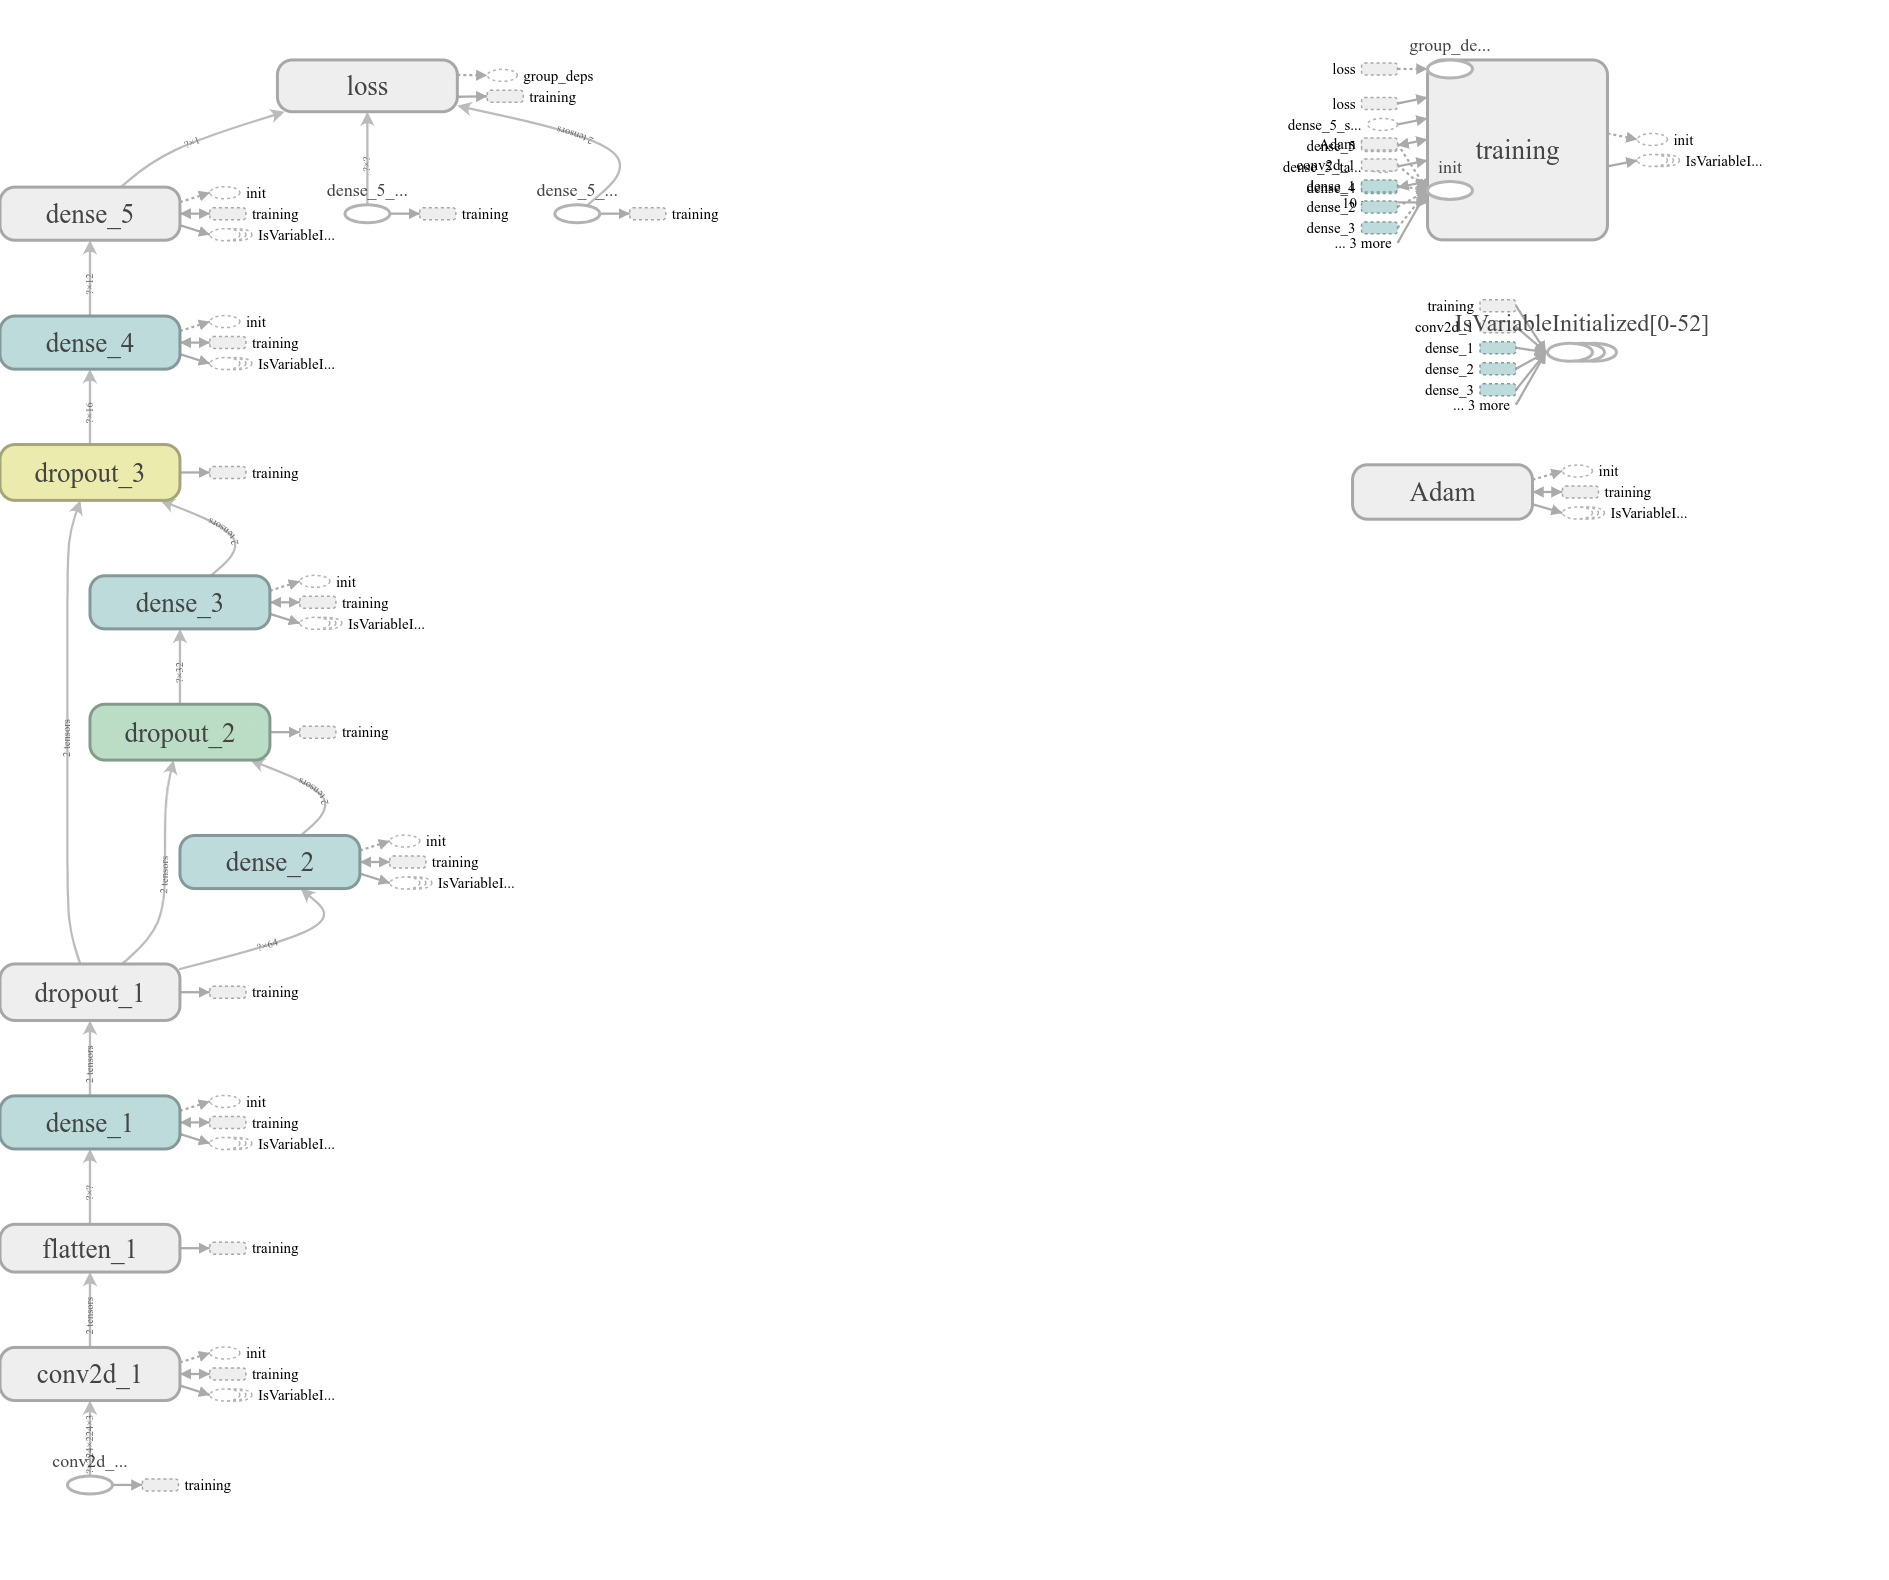
\includegraphics[width=0.9\textwidth]{../img/arqdense}
    \end{figure}

\end{frame}



\begin{frame}{Red neuronal convolucional}
    \begin{table}[!h]
        \centering
        \resizebox{0.9\textwidth}{!}{%
        \begin{tabular}{@{}cccccc@{}}
        \toprule
        \multicolumn{1}{|c|}{\textbf{Capa}}     & \multicolumn{1}{c|}{\textbf{Tipo}} & \multicolumn{1}{c|}{\textbf{\begin{tabular}[c]{@{}c@{}}Unidades\\ (Filtros)\end{tabular}}} & \multicolumn{1}{c|}{\textbf{\begin{tabular}[c]{@{}c@{}}Dimensiones \\ de salida\end{tabular}}} & \multicolumn{1}{c|}{\textbf{\begin{tabular}[c]{@{}c@{}}Parámetros \\ entrenables\end{tabular}}} & \multicolumn{1}{c|}{\textbf{\begin{tabular}[c]{@{}c@{}}Función de \\ Activación\end{tabular}}} \\ \midrule
        \multicolumn{1}{|c|}{input\_1}          & \multicolumn{1}{c|}{InputLayer}    & \multicolumn{1}{c|}{-}                                                                     & \multicolumn{1}{c|}{(224,224,3)}                                                               & \multicolumn{1}{c|}{0}                                                                          & \multicolumn{1}{c|}{}                                                                          \\ \midrule
        \multicolumn{1}{|c|}{conv2d\_1}         & \multicolumn{1}{c|}{Conv2D}        & \multicolumn{1}{c|}{16 (3 x 5)}                                                            & \multicolumn{1}{c|}{(222,220,16)}                                                              & \multicolumn{1}{c|}{736}                                                                        & \multicolumn{1}{c|}{ReLU}                                                                      \\ \midrule
        \multicolumn{1}{|c|}{conv2d\_2}         & \multicolumn{1}{c|}{Conv2D}        & \multicolumn{1}{c|}{16 (3 x 5)}                                                            & \multicolumn{1}{c|}{(220,216,16)}                                                              & \multicolumn{1}{c|}{3856}                                                                       & \multicolumn{1}{c|}{ReLU}                                                                      \\ \midrule
        \multicolumn{1}{|c|}{max\_pooling2d\_1} & \multicolumn{1}{c|}{MaxPooling2D}  & \multicolumn{1}{c|}{-}                                                                     & \multicolumn{1}{c|}{(55,108,16)}                                                               & \multicolumn{1}{c|}{-}                                                                          & \multicolumn{1}{c|}{-}                                                                         \\ \midrule
        \multicolumn{1}{|c|}{conv2d\_3}         & \multicolumn{1}{c|}{Conv2D}        & \multicolumn{1}{c|}{32 (3 x 5)}                                                            & \multicolumn{1}{c|}{(53,104,32)}                                                               & \multicolumn{1}{c|}{7712}                                                                       & \multicolumn{1}{c|}{ReLU}                                                                      \\ \midrule
        \multicolumn{1}{|c|}{conv2d\_4}         & \multicolumn{1}{c|}{Conv2D}        & \multicolumn{1}{c|}{32 (3 x 5)}                                                            & \multicolumn{1}{c|}{(51,100,32)}                                                               & \multicolumn{1}{c|}{15392}                                                                      & \multicolumn{1}{c|}{ReLU}                                                                      \\ \midrule
        \multicolumn{1}{|c|}{max\_pooling2d\_2} & \multicolumn{1}{c|}{MaxPooling2D}  & \multicolumn{1}{c|}{-}                                                                     & \multicolumn{1}{c|}{(12,50,32)}                                                                & \multicolumn{1}{c|}{-}                                                                          & \multicolumn{1}{c|}{-}                                                                         \\ \midrule
        \multicolumn{1}{|c|}{conv2d\_5}         & \multicolumn{1}{c|}{Conv2D}        & \multicolumn{1}{c|}{64 (3 x 5)}                                                            & \multicolumn{1}{c|}{(10,46,64)}                                                                & \multicolumn{1}{c|}{30784}                                                                      & \multicolumn{1}{c|}{ReLU}                                                                      \\ \midrule
        \multicolumn{1}{|c|}{conv2d\_6}         & \multicolumn{1}{c|}{Conv2D}        & \multicolumn{1}{c|}{64 (3 x 5)}                                                            & \multicolumn{1}{c|}{(8,42,64)}                                                                 & \multicolumn{1}{c|}{61504}                                                                      & \multicolumn{1}{c|}{ReLU}                                                                      \\ \midrule
        \multicolumn{1}{|c|}{max\_pooling2d\_3} & \multicolumn{1}{c|}{MaxPooling2D}  & \multicolumn{1}{c|}{-}                                                                     & \multicolumn{1}{c|}{(2,21,64)}                                                                 & \multicolumn{1}{c|}{-}                                                                          & \multicolumn{1}{c|}{-}                                                                         \\ \midrule
        \multicolumn{1}{|c|}{conv2d\_7}         & \multicolumn{1}{c|}{Conv2D}        & \multicolumn{1}{c|}{64 (3 x 5)}                                                            & \multicolumn{1}{c|}{(2,21,4)}                                                                  & \multicolumn{1}{c|}{260}                                                                        & \multicolumn{1}{c|}{ReLU}                                                                      \\ \midrule
        \multicolumn{1}{|c|}{dense\_1}          & \multicolumn{1}{c|}{Dense}         & \multicolumn{1}{c|}{1}                                                                     & \multicolumn{1}{c|}{1}                                                                         & \multicolumn{1}{c|}{169}                                                                        & \multicolumn{1}{c|}{Tanh}                                                                      \\ \midrule
                                                &                                    &                                                                                            &                                                                                                &                                                                                                 &                                                                                                \\ \cmidrule(l){3-6} 
                                                & \multicolumn{1}{c|}{}              & \multicolumn{2}{c|}{Total Capas}                                                                                                                                                            & \multicolumn{2}{c|}{12}                                                                                                                                                                          \\ \cmidrule(l){3-6} 
                                                & \multicolumn{1}{c|}{}              & \multicolumn{2}{c|}{Total Parámetros}                                                                                                                                                       & \multicolumn{2}{c|}{120413}                                                                                                                                                                      \\ \cmidrule(l){3-6} 
        \end{tabular}%
        }
    \end{table}

\end{frame}

\begin{frame}{Red neuronal convolucional}
    \begin{figure}[!h] 
        \centering
        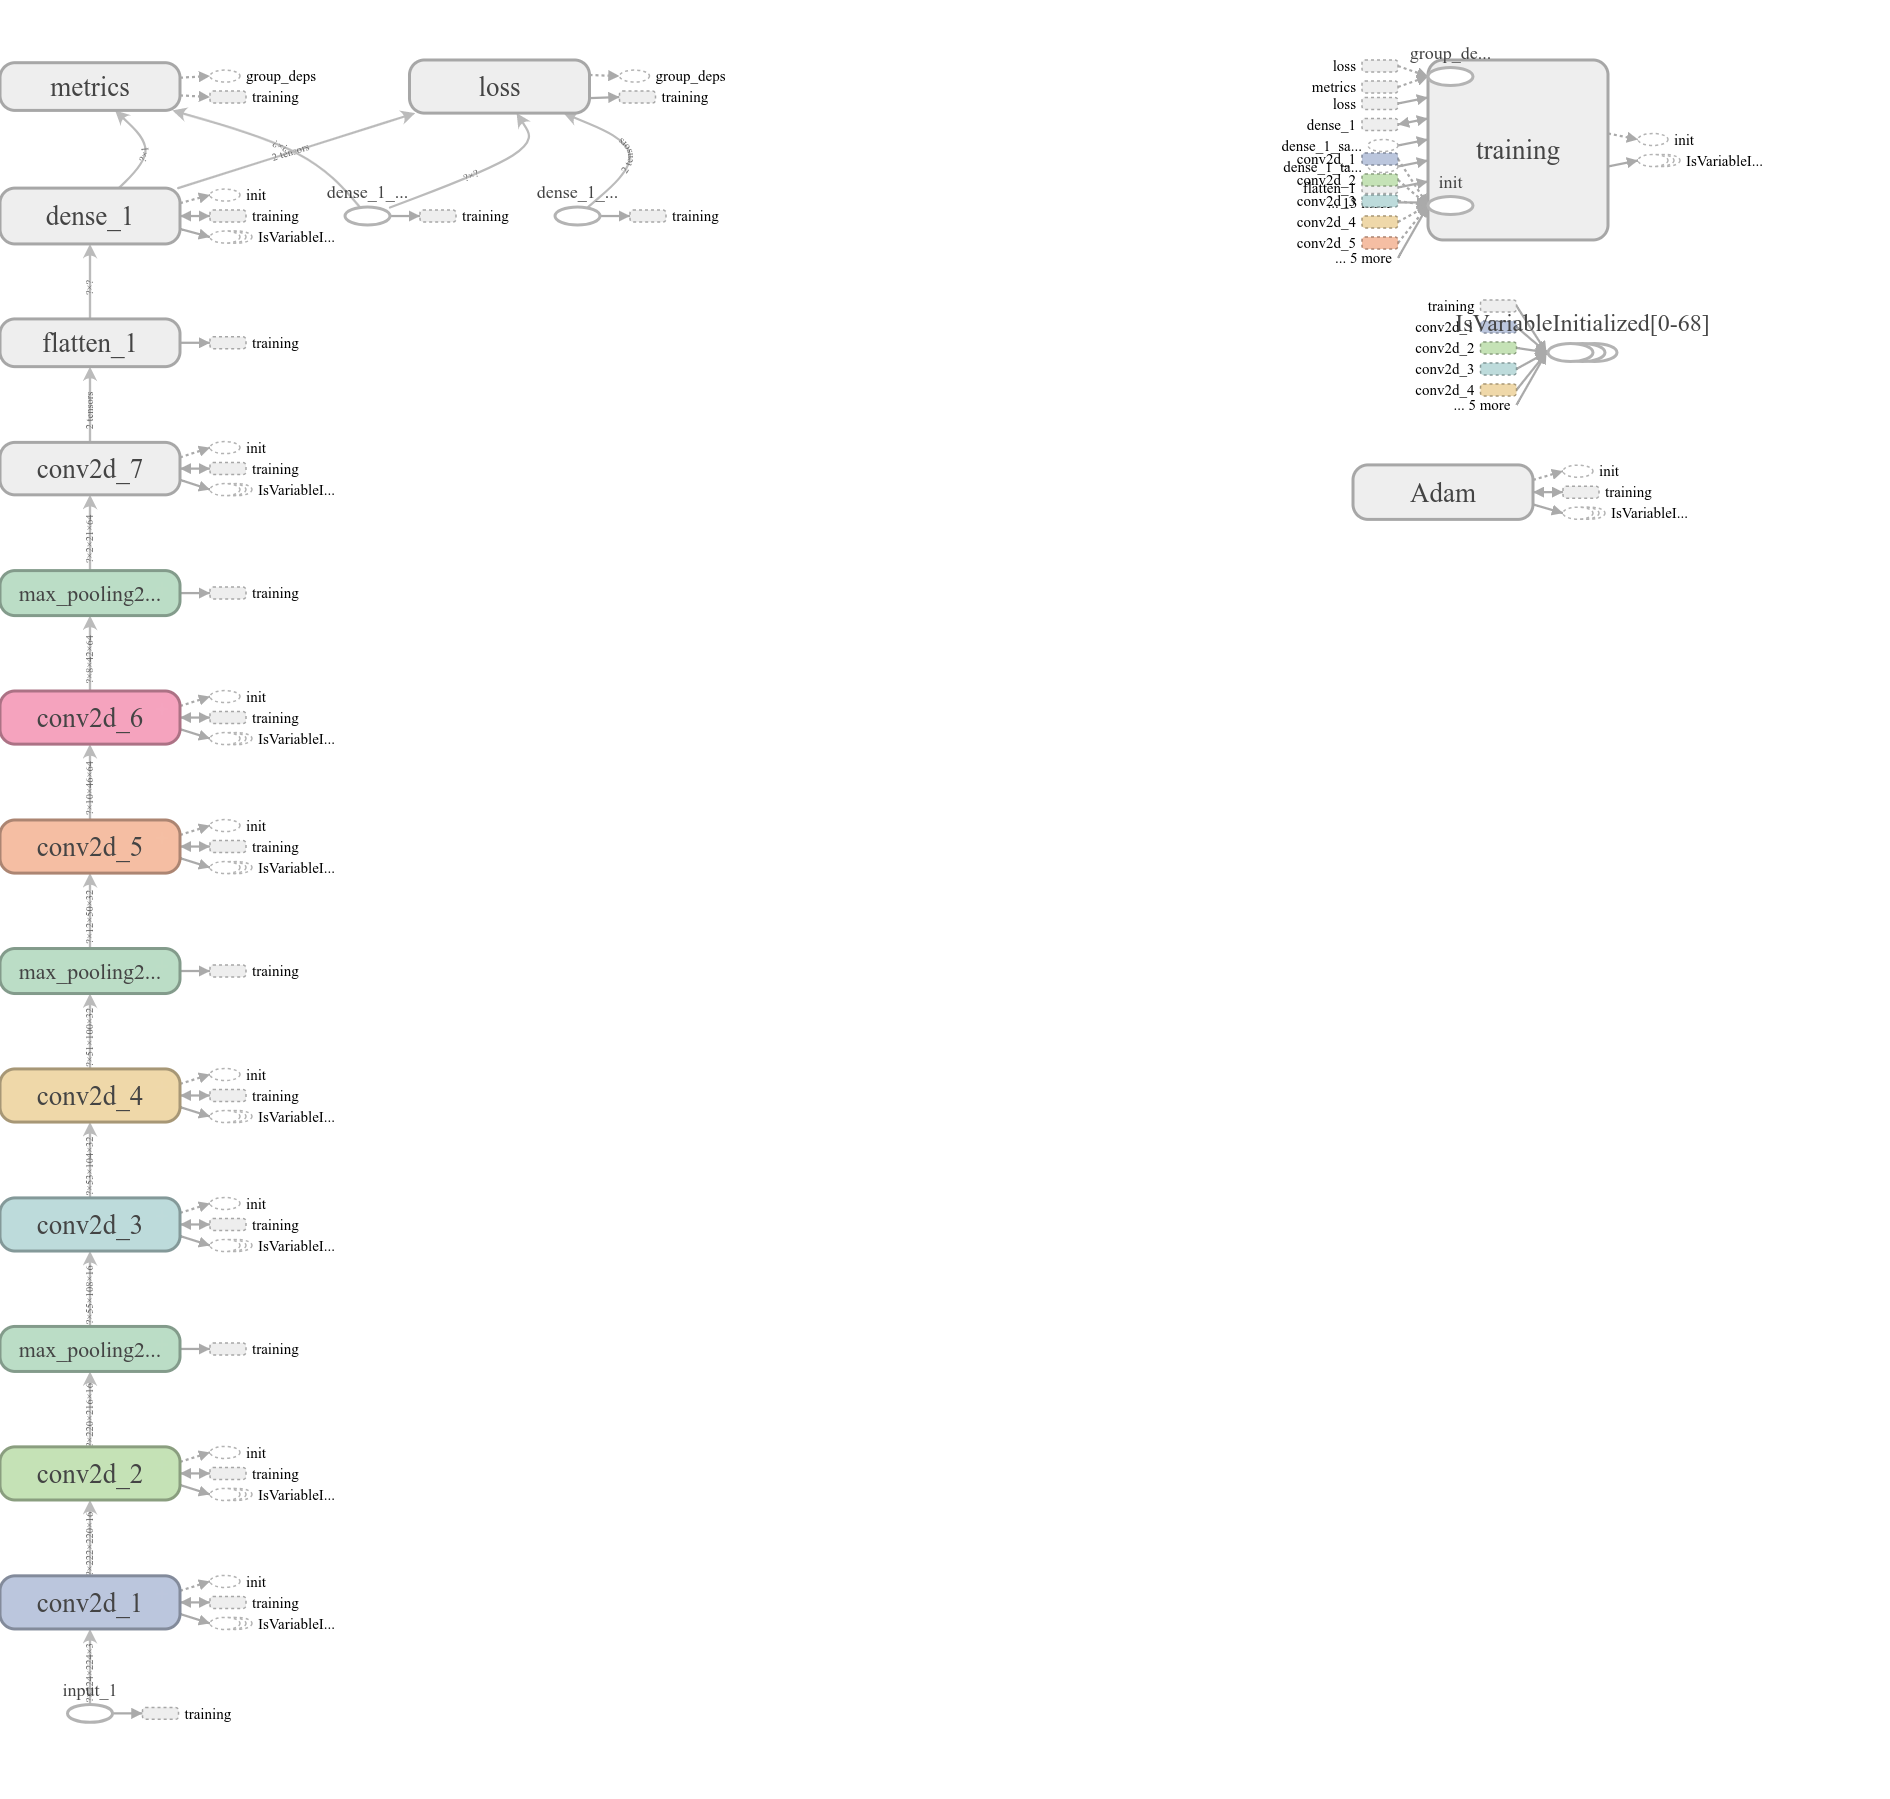
\includegraphics[width=0.8\textwidth]{../img/arqconv}   
    \end{figure}
\end{frame}

\section*{Conjunto de datos}

\begin{frame}{Balanceo del conjunto de datos}
    Debido a la naturaleza de las sesiones de entrenamiento, el conjunto de datos inicial 
    se encuentra desbalanceado.
    \begin{figure}[!h] 
        \centering
        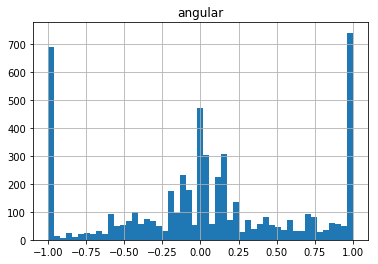
\includegraphics[width=0.65\textwidth]{../img/histinicial}
        \caption[Distribución inicial del dataset]{Distribución inicial del dataset. Fuente: Elaboración propia. }
        \label{fig:histinicial}
    \end{figure}
\end{frame}

\begin{frame}{Balanceo del conjunto de datos}
    Se procede a realizar un balanceo del conjunto en base a dos tareas fundamentales:
    \begin{itemize}
        \item Eliminación de muestras con valor muy cercano o igual a cero.
        \item Aumentación de muestras con transformaciones aleatorias.
    \end{itemize}
\end{frame}

\begin{frame}{Balanceo del conjunto de datos}
    Una vez realizadas las operaciones se tiene un conjunto de datos con la siguiente distribución:
    \begin{figure}[!h] 
        \centering
        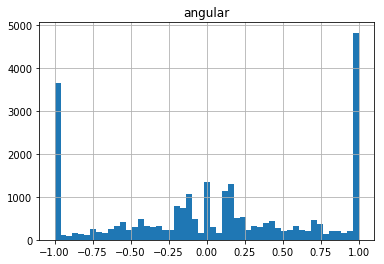
\includegraphics[width=0.65\textwidth]{../img/histfinal}
        \caption[Distribución final del dataset]{Distribución final del dataset. Fuente: Elaboración propia. }
        \label{fig:histfinal}
    \end{figure}
\end{frame}


\begin{frame}{Separación de conjuntos de datos}
    
    \begin{columns}
        \begin{column}{0.5\textwidth}
            Se ha separado el conjunto de datos en tres conjuntos con funciones distintas:
            \begin{itemize}
                \item \alert{Entrenamiento}: Datos sobre los que se entrena la red neuronal en cada época.
                \item \alert{Validación}: Pequeño conjunto sobre el cual se evalúa el error entre épocas.
                \item \alert{Pruebas}: Conjunto no presente en el entrenamiento sobre el cual se realizan pruebas de rendimiento.
            \end{itemize} 
        \end{column}
        \begin{column}{0.5\textwidth}
            \begin{table}[!h]
                \centering
                \resizebox{0.75\textwidth}{!}{%
                \begin{tabular}{@{}|l|l|l|@{}}
                    \toprule
                    \textbf{Conjunto de datos} & \textbf{Muestras} & \textbf{Fracción} \\ \midrule
                    Entrenamiento              & 21084             & 80\%              \\ \midrule
                    Prueba                     & 3691              & 16\%              \\ \midrule
                    Validación                 & 1581              & 4\%               \\ \midrule
                    \textbf{Total}             & \textbf{26356}    & \textbf{100\%}    \\ \bottomrule
                    \end{tabular}%
                    }
            \end{table}
            \begin{figure}[!h] 
                \centering
                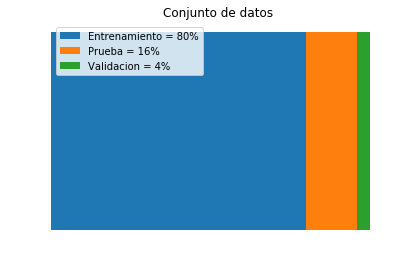
\includegraphics[width=\textwidth]{../img/dataset1}
            \end{figure}
        \end{column}
    \end{columns}
    
\end{frame}

% \begin{frame}{Separación de conjuntos de datos}
%     \begin{table}[!h]
%         \centering
%         \resizebox{0.5\textwidth}{!}{%
%         \begin{tabular}{@{}|l|l|l|@{}}
%             \toprule
%             \textbf{Conjunto de datos} & \textbf{Muestras} & \textbf{Fracción} \\ \midrule
%             Entrenamiento              & 21084             & 80\%              \\ \midrule
%             Prueba                     & 3691              & 16\%              \\ \midrule
%             Validación                 & 1581              & 4\%               \\ \midrule
%             \textbf{Total}             & \textbf{26356}    & \textbf{100\%}    \\ \bottomrule
%             \end{tabular}%
%             }
%     \end{table}
%     \begin{figure}[!h] 
%         \centering
%         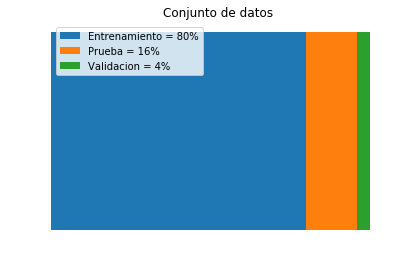
\includegraphics[width=0.65\textwidth]{../img/dataset1}
%     \end{figure}
% \end{frame}


\section{Análisis de Resultados}

\section*{Entrenamiento}

\begin{frame}{Error de Entrenamiento}
    \begin{figure}[!ht] 
        \centering
        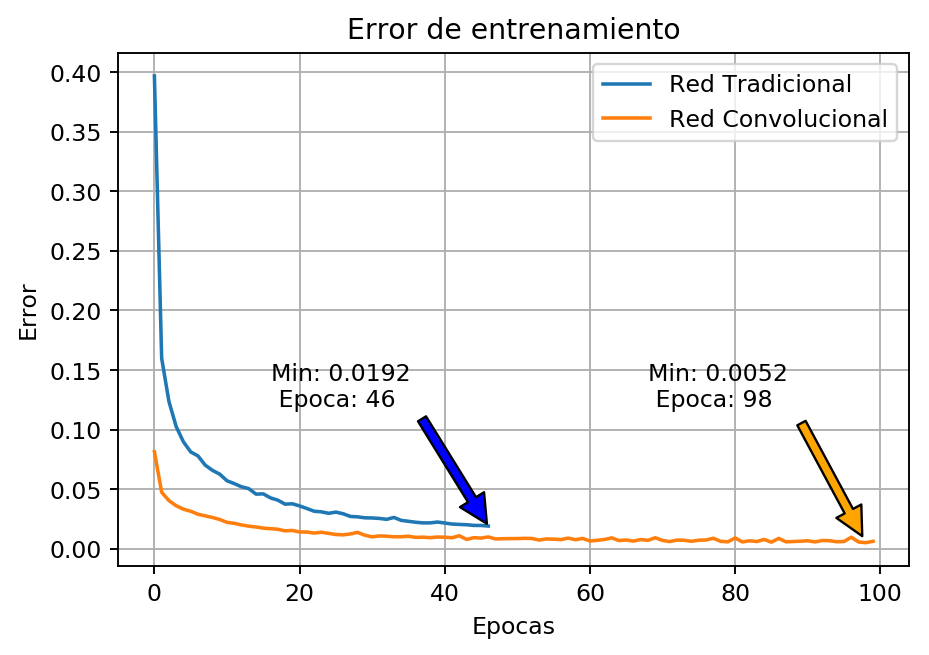
\includegraphics[width=0.75\textwidth]{../img/trainloss}
        \caption[Error de entrenamiento]{Error de entrenamiento. Fuente: Elaboración propia. }
        \label{fig:trainloss}
    \end{figure}
    
\end{frame}

% \begin{frame}{Error de Entrenamiento}
%     \begin{itemize}
%         \item \textbf{El error de entrenamiento inicial es menor:} La capacidad de ajuste de parámetros 
%         es más eficaz en la red neuronal convolucional.
%         \item \textbf{El error mínimo es menor:} La red convolucional se aproxima mejor al conjunto de 
%         entrenamiento.
%         \item \textbf{Convergencia más rápida:} La velocidad de convergencia hacia el valor mínimo es casi el doble. La convergencia está directamente 
%         relacionada con el tiempo de entrenamiento requerido por cada arquitectura.
%     \end{itemize}
    
% \end{frame}

\begin{frame}{Error de Validación}
    \begin{figure}[!ht] 
        \centering
        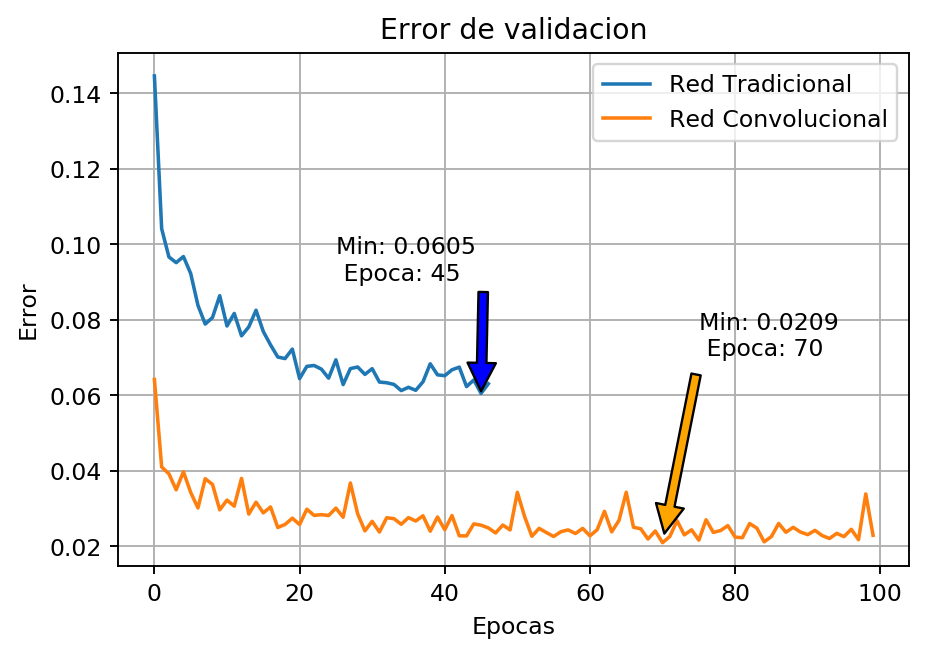
\includegraphics[width=0.75\textwidth]{../img/valloss}
        \caption[Error de validación]{Error de validación. Fuente: Elaboración propia. }
        \label{fig:valloss}
    \end{figure}
    
\end{frame}


% \begin{frame}{Error de Validación}
%     \begin{itemize}
%         \item \textbf{El error de inicial es menor:} Con solamente una pasada por el conjunto de entrenamiento, se tiene una 
%         capacidad mayor de realizar predicciones cercanas a la realidad en casos nunca antes vistos.
%         \item \textbf{El error mínimo es menor:} La capacidad de generalización 
%         de la red convolucional es mayor al de la red tradicional. Si el error de la red convolucional fuera mayor, esto podría indicar 
%         sobreentrenamiento de la red.
%         \item \textbf{Convergencia:} Los valores del error son menores para la red convolucional mostrando que su rendimiento 
%         y capacidad de generalización son mayores al de una red tradicional.
%     \end{itemize}
    
% \end{frame}
\section*{Pruebas}
\begin{frame}{Puntajes y errores en el conjunto de prueba}
    \begin{columns}
        \begin{column}{0.4\textwidth}
            \small{Los puntajes sobre el conjunto de prueba definen el rendimiento y la capacidad de generalización de la 
            red sobre datos nunca antes vistos. Se usan las siguientes métricas:}
    
            \begin{itemize}
                \item \alert{MSE}: Error Cuadrático Medio.
                \item \alert{MAE}: Error Absoluto Medio.
                \item \alert{$R^2$}: Coeficiente de Determinación.
            \end{itemize}
        \end{column}
        \begin{column}{0.6\textwidth}
            \begin{table}[!h]
                \centering
                \resizebox{0.95\textwidth}{!}{%
                \begin{tabular}{@{}|c|c|c|c|@{}}
                \toprule
                \textbf{Modelo} & \textbf{MSE} & \textbf{MAE} & $\mathbf{R^2}$ \\ \midrule
                Tradicional & 0.0254 & 0.0976 & 0.9278 \\ \midrule
                Convolucional & 0.0160 & 0.0872 & 0.9484 \\ \bottomrule
                \end{tabular}%
                }
                \caption[Evaluación de puntajes sobre el conjunto de prueba.]{Evaluación de puntajes sobre el conjunto de prueba. Fuente: Elaboración propia.}
                \label{tbl:testscores}
            \end{table}
        \end{column}
    \end{columns}
    

\end{frame}

% \begin{frame}{Puntajes y errores en el conjunto de prueba}
%     \begin{table}[!h]
%         \centering
%         \resizebox{0.65\textwidth}{!}{%
%         \begin{tabular}{@{}|c|c|c|c|@{}}
%         \toprule
%         \textbf{Modelo} & \textbf{MSE} & \textbf{MAE} & $\mathbf{R^2}$ \\ \midrule
%         Tradicional & 0.0254 & 0.0976 & 0.9278 \\ \midrule
%         Convolucional & 0.0160 & 0.0872 & 0.9484 \\ \bottomrule
%         \end{tabular}%
%         }
%         \caption[Evaluación de puntajes sobre el conjunto de prueba.]{Evaluación de puntajes sobre el conjunto de prueba. Fuente: Elaboración propia.}
%         \label{tbl:testscores}
%     \end{table}

% \end{frame}

\begin{frame}{Puntajes y errores en el conjunto de prueba}
    \begin{table}[]
        \centering
        \resizebox{0.75\textwidth}{!}{%
        \begin{tabular}{@{}|c|c|c|c|@{}}
        \toprule
        \textbf{Valor real} & \textbf{Predicción} & \textbf{Diferencia} & \textbf{\begin{tabular}[c]{@{}c@{}}Predicción de\\ signo correcta\end{tabular}} \\ \midrule
        -0.297 & -0.243 & 0.054 & \checkmark \\ \midrule
        1.0 & 0.921 & 0.079 & \checkmark \\ \midrule
        0.149 & 0.22 & 0.07 & \checkmark \\ \midrule
        -1. & -0.968 & 0.032 & \checkmark \\ \midrule
        -0. & 0.069 & 0.069 & $\times$ \\ \bottomrule
        \end{tabular}%
        }
        \caption[Muestra de predicciones de la red convolucional.]{Muestra de predicciones de la red convolucional. Fuente: Elaboración propia.}
        \label{tbl:predsample}
    \end{table}

\end{frame}

\begin{frame}{Pruebas de Campo}
    \begin{figure}[!h] 
        \centering
        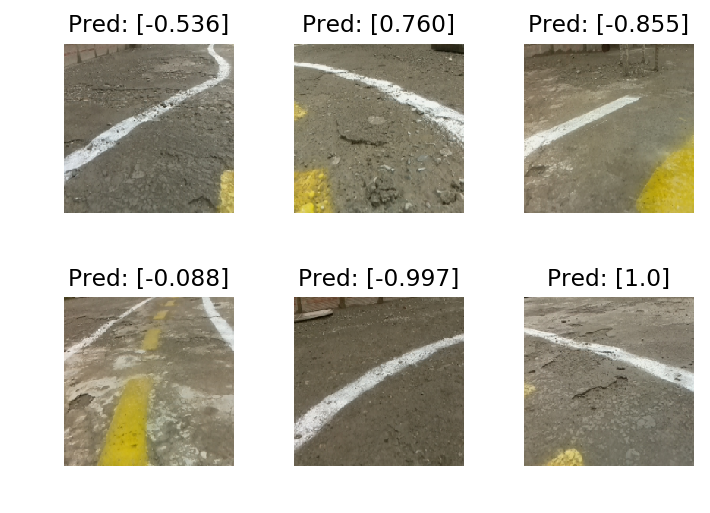
\includegraphics[width=0.75\textwidth]{../img/testimg}
        \caption[Ejemplos de predicción de la red convolucional]{Ejemplos de predicción de la red convolucional. Fuente: Elaboración propia. }
        \label{fig:testimg}
    \end{figure}
\end{frame}

\begin{frame}{Representaciones Internas}
    \begin{figure}[!h] 
        \centering
        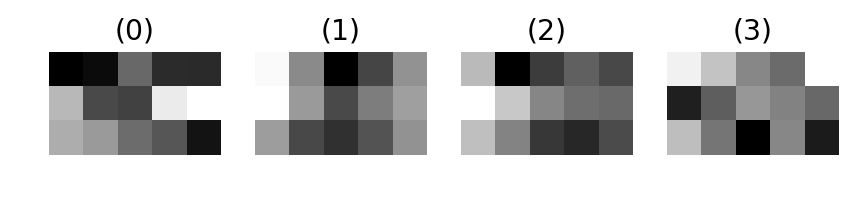
\includegraphics[width=0.65\textwidth]{../img/filtros7}
        \caption[Filtros de la penúltima capa convolucional]{Filtros de la penúltima capa convolucional. Fuente: Elaboración propia. }
        \label{fig:filtros7}
    \end{figure}
    \begin{figure}[!h] 
        \centering
        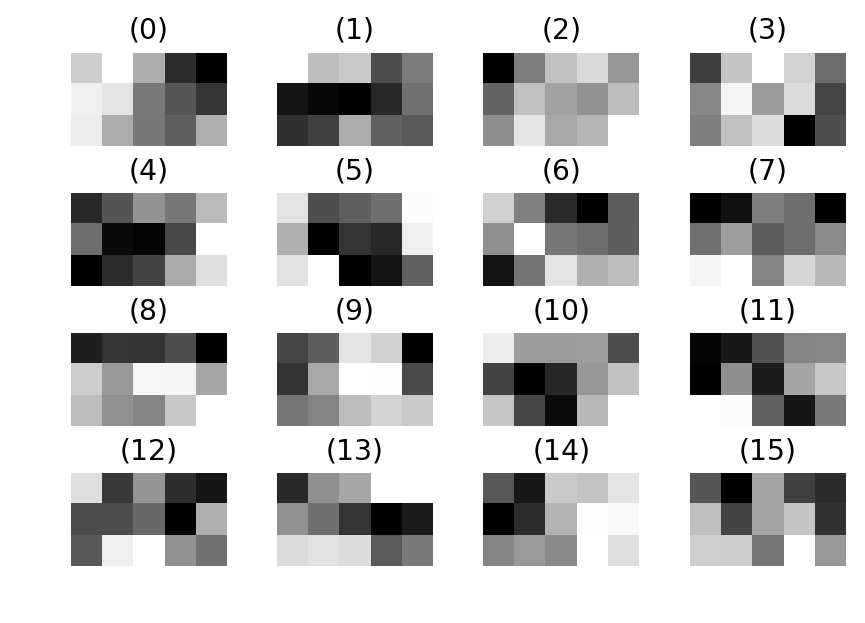
\includegraphics[width=0.45\textwidth]{../img/filtros1}
        \caption[Filtros de la primera capa convolucional]{Filtros de la primera capa convolucional. Fuente: Elaboración propia. }
        \label{fig:filtros1}
    \end{figure}
\end{frame}

% \begin{frame}{Representaciones Internas}
%     \begin{figure}[!h] 
%         \centering
%         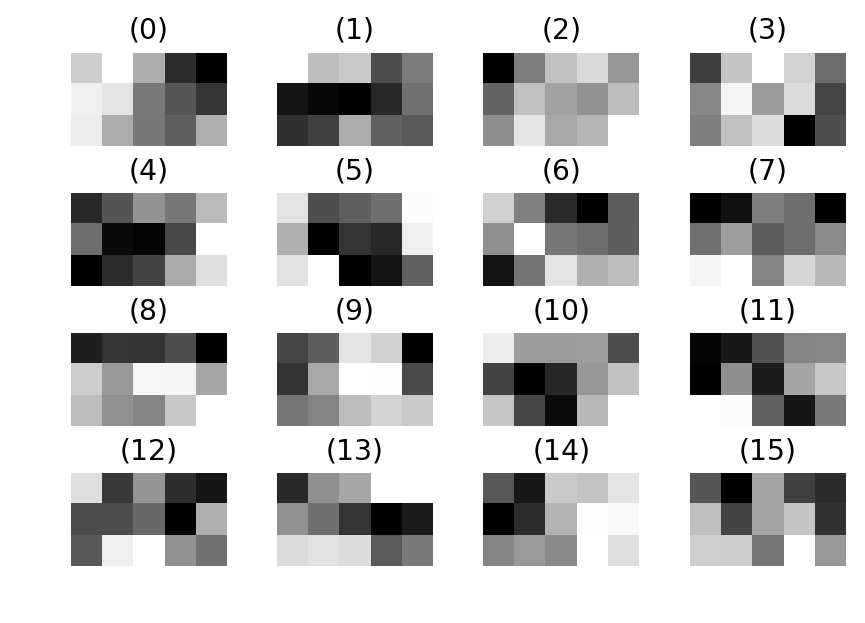
\includegraphics[width=0.65\textwidth]{../img/filtros1}
%         \caption[Filtros de la primera capa convolucional]{Filtros de la primera capa convolucional. Fuente: Elaboración propia. }
%         \label{fig:filtros1}
%     \end{figure}
% \end{frame}

\begin{frame}{Representaciones Internas}
    \begin{columns}
        
        \begin{column}{0.31\textwidth}
            Giro a la izquierda. Predicción: \alert{1}.
            \begin{figure}[!h] 
                \centering
                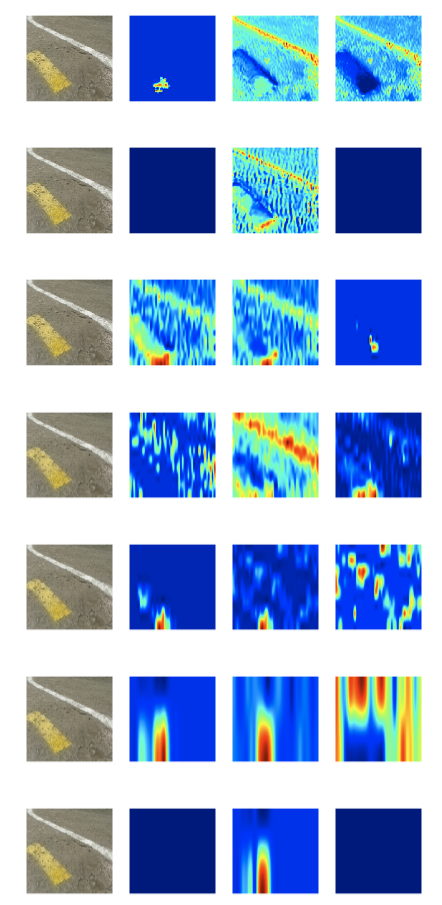
\includegraphics[width=\textwidth]{../img/predizq}
            \end{figure}
        \end{column}
        
        \begin{column}{0.31\textwidth}
            Hacia adelante. Predicción: \alert{-0.1}.
            \begin{figure}[!h] 
                \centering
                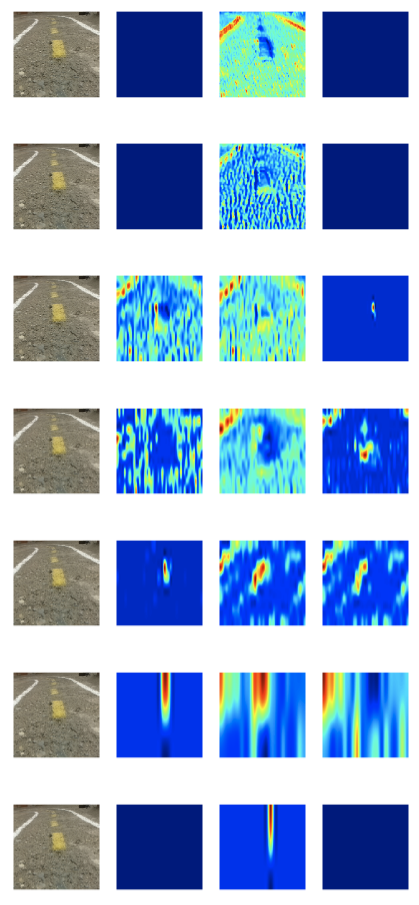
\includegraphics[width=0.95\textwidth]{../img/predade}
            \end{figure}
        \end{column}
        
        \begin{column}{0.31\textwidth}
            Giro a la derecha. Predicción: \alert{-0.84}.
            \begin{figure}[!h] 
                \centering
                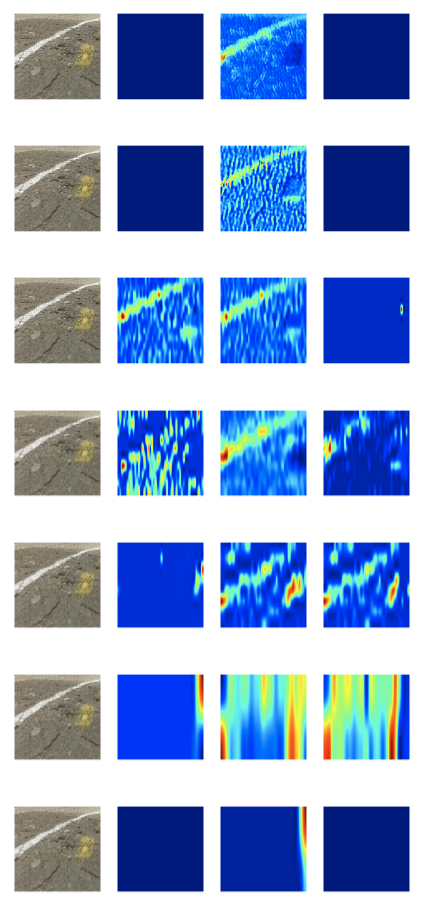
\includegraphics[width=0.97\textwidth]{../img/predder}
            \end{figure}
        \end{column}
    \end{columns}
\end{frame}


% \begin{frame}{Representaciones Internas}
%     Giro a la izquierda. Predicción: \alert{1}.
%     \begin{figure}[!h] 
%         \centering
%         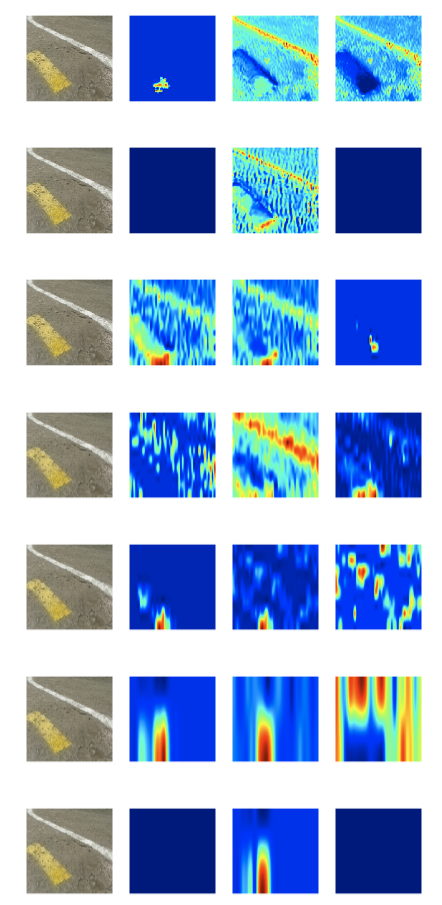
\includegraphics[width=0.33\textwidth]{../img/predizq}
%     \end{figure}
% \end{frame}

% \begin{frame}{Representaciones Internas}
%     Giro a la derecha. Predicción: \alert{-0.84}.
%     \begin{figure}[!h] 
%         \centering
%         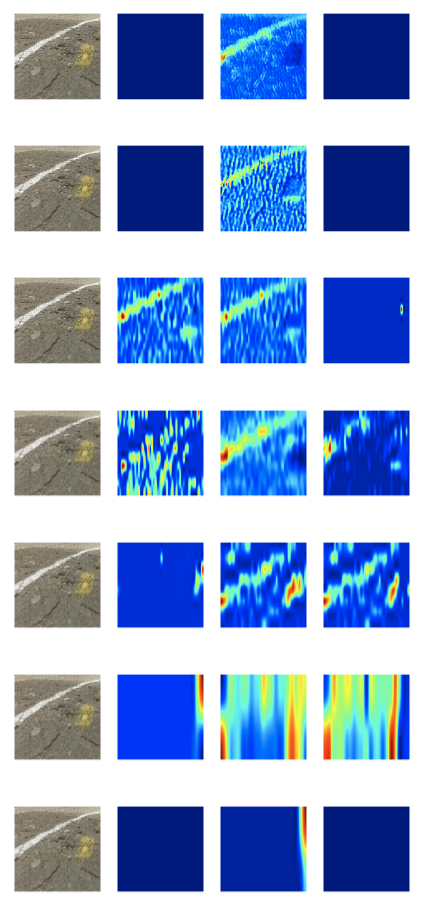
\includegraphics[width=0.33\textwidth]{../img/predder}
%     \end{figure}
% \end{frame}

% \begin{frame}{Representaciones Internas}
%     Conducción hacia adelante. Predicción: \alert{-0.1}.
%     \begin{figure}[!h] 
%         \centering
%         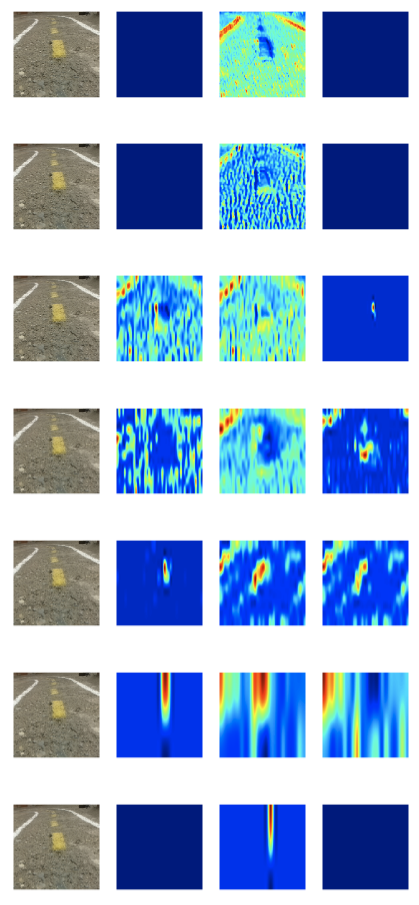
\includegraphics[width=0.33\textwidth]{../img/predade}
%     \end{figure}
% \end{frame}

\section{Conclusiones y Recomendaciones}

\begin{frame}[allowframebreaks]{Conclusiones}
    \begin{itemize}
        \item \alert{Se estudiaron} los aspectos relacionados al desarrollo de sistemas de conducción autónoma, y posteriormente los conceptos básicos 
        de aprendizaje automático, aprendizaje profundo, redes convolucionales y el proceso de entrenamiento de una red neuronal.
        \item Se ha introducido el \alert{esquema de la arquitectura} de un sistema de conducción autónomo y se han planteado 
        los requisitos y funcionalidades que debe tener el sistema en su conjunto y por cada subsistema y módulos correspondientes.
        \item \alert{Se han diseñado} todos los subsistemas correspondientes en base a las limitaciones y herramientas de software y hardware elegidas. Los subsistemas son:
            \begin{itemize}
                \item Subsistema de Control y Actuación.
                \item Subsistema de Adquisición de Datos y Entrenamiento.
                \item Subsistema de Inferencia y Control Autónomo
            \end{itemize}
            \item \alert{Se ha implementado} una red neuronal convolucional para la tarea de la conducción autónoma.
            \item \alert{Se ha entrenado} de manera satisfactoria una red neuronal convolucional.
            \item \alert{Se ha validado el rendimiento} de la red neuronal convolucional para tareas de visión artificial en base a una comparación con otra arquitectura tradicional.
        
    \end{itemize}
\end{frame}


\begin{frame}[allowframebreaks]{Recomendaciones}
    \begin{itemize}
        \item Generar \alert{distintos conjuntos} de entrenamiento en condiciones climáticas diversas y ambientes variados. 
        \item Diseñar, entrenar y validar arquitecturas de \alert{redes neuronales distintas} o con variaciones a una red neuronal convolucional 
        tradicional.
        \item Extender la implementación de la red a una tarea de \alert{clasificación categórica}.
        \item Implementar el sistema desarrollado en \alert{otros modelos de vehículos}, como por ejemplo, tracción diferencial.
        \item Extender el sistema presentado en este proyecto con \alert{tareas avanzadas}, incluyendo en el flujo de trabajo, módulos de planificación de trayectorias, detección de objetos y 
        programación de misiones.
        \item Crear una \alert{línea de investigación} dedicada al diseño e implementación de sistemas robóticos inteligentes y vehículos autónomos en el IEA.
        \item Considerar este proyecto y sus resultados como una \alert{plataforma de desarrollo} sobre la cual se puedan implementar diversos algoritmos y aplicaciones en sistemas robóticos inteligentes y vehículos autónomos.
    
    \end{itemize}
    
\end{frame}

% {%
% \setbeamertemplate{frame footer}{My custom footer}
% \begin{frame}[fragile]{Frame footer}
%     \themename defines a custom beamer template to add a text to the footer. It can be set via
%     \begin{verbatim}\setbeamertemplate{frame footer}{My custom footer}\end{verbatim}
% \end{frame}
% }

{\setbeamercolor{palette primary}{fg=black, bg=yellow}
\begin{frame}[standout]
  Preguntas?
\end{frame}
}

\appendix

% \begin{frame}[fragile]{Backup slides}
%   Sometimes, it is useful to add slides at the end of your presentation to
%   refer to during audience questions.

%   The best way to do this is to include the \verb|appendixnumberbeamer|
%   package in your preamble and call \verb|\appendix| before your backup slides.

%   \themename will automatically turn off slide numbering and progress bars for
%   slides in the appendix.
% \end{frame}

\begin{frame}[allowframebreaks]{Referencias}

  \bibliography{../referencias}
  \bibliographystyle{IEEEtran}

\end{frame}

\end{document}
